%%%%%%%%%%%%%%%%%%%%%%%%%%%%%%%%%%%%%%%%%
% Arsclassica Article
% LaTeX Template
% Version 1.1 (1/8/17)
%
% This template has been downloaded from:
% http://www.LaTeXTemplates.com
%
% Original author:
% Lorenzo Pantieri (http://www.lorenzopantieri.net) with extensive modifications by:
% Vel (vel@latextemplates.com)
%
% License:
% CC BY-NC-SA 3.0 (http://creativecommons.org/licenses/by-nc-sa/3.0/)
%
%%%%%%%%%%%%%%%%%%%%%%%%%%%%%%%%%%%%%%%%%

%----------------------------------------------------------------------------------------
%	PACKAGES AND OTHER DOCUMENT CONFIGURATIONS
%----------------------------------------------------------------------------------------

\documentclass[
12pt, % Main document font size
a4paper, % Paper type, use 'letterpaper' for US Letter paper
oneside, % One page layout (no page indentation)
%twoside, % Two page layout (page indentation for binding and different headers)
headinclude,footinclude, % Extra spacing for the header and footer
BCOR5mm, % Binding correction
]{scrartcl}
\usepackage[english]{babel}
\usepackage{url}
\usepackage{graphicx}
\usepackage{calligra}
\usepackage[T1]{fontenc}
\usepackage{subcaption}
\usepackage{float}
\usepackage{afterpage}
\usepackage{titlepic}
\usepackage{epigraph}
\usepackage{mathcomp}
\usepackage{textcomp}
\usepackage{placeins}
\usepackage{mathtools}
\usepackage[LGR,T1]{fontenc}
\usepackage{amsmath}
\usepackage{url}
\usepackage{sectsty}
\usepackage[dvipsnames,table,xcdraw,svgnames]{xcolor}
\usepackage{listings}
\usepackage{booktabs}
\usepackage{lipsum}
\newcommand{\textgreek}[1]{\begingroup\fontencoding{LGR}\selectfont#1\endgroup}
\usepackage{url}
\lstset{language=R,
    basicstyle=\small\ttfamily,
    stringstyle=\color{DarkGreen},
    otherkeywords={0,1,2,3,4,5,6,7,8,9},
    morekeywords={TRUE,FALSE},
    deletekeywords={data,frame,length,as,character},
    keywordstyle=\color{blue},
    commentstyle=\color{DarkGreen},
}
\usepackage[pdftex,
            pdfauthor={Marzio De Corato},
            pdftitle={A bird's-eye view on the habitability of exoplanets via statistical learning techniques},
            pdfsubject={Project for the exam: Machine learning, statistical learning, deep learning and artificial intelligenc},
            pdfproducer={Latex},
            pdfcreator={pdflatex}]{hyperref}
            

%%%%%%%%%%%%%%%%%%%%%%%%%%%%%%%%%%%%%%%%%
% Arsclassica Article
% Structure Specification File
%
% This file has been downloaded from:
% http://www.LaTeXTemplates.com
%
% Original author:
% Lorenzo Pantieri (http://www.lorenzopantieri.net) with extensive modifications by:
% Vel (vel@latextemplates.com)
%
% License:
% CC BY-NC-SA 3.0 (http://creativecommons.org/licenses/by-nc-sa/3.0/)
%
%%%%%%%%%%%%%%%%%%%%%%%%%%%%%%%%%%%%%%%%%

%----------------------------------------------------------------------------------------
%	REQUIRED PACKAGES
%----------------------------------------------------------------------------------------

\usepackage[
nochapters, % Turn off chapters since this is an article        
beramono, % Use the Bera Mono font for monospaced text (\texttt)
eulermath,% Use the Euler font for mathematics
pdfspacing, % Makes use of pdftex’ letter spacing capabilities via the microtype package
dottedtoc % Dotted lines leading to the page numbers in the table of contents
]{classicthesis} % The layout is based on the Classic Thesis style

\usepackage{arsclassica} % Modifies the Classic Thesis package

\usepackage[T1]{fontenc} % Use 8-bit encoding that has 256 glyphs

\usepackage[utf8]{inputenc} % Required for including letters with accents

\usepackage{graphicx} % Required for including images
\graphicspath{{Figures/}} % Set the default folder for images
 % Include the structure.tex file which specified the document structure and layout
\sloppy
\hyphenation{Fortran hy-phen-ation} % Specify custom hyphenation points in words with dashes where you would like hyphenation to occur, or alternatively, don't put any dashes in a word to stop hyphenation altogether

%----------------------------------------------------------------------------------------
%	TITLE AND AUTHOR(S)
%----------------------------------------------------------------------------------------

\begin{document}




\title{\normalfont{A bird's-eye view on the habitability of exoplanets via statistical learning techniques}} % The article title

\subtitle{Project for the exam: Machine learning, statistical learning, deep learning and artificial intelligence} % Uncomment to display a subtitle


\author{Marzio De Corato} % The article author(s) - author affiliations need to be specified in the AUTHOR AFFILIATIONS block

\date{\today} % An optional date to appear under the author(s)

%\titlepic{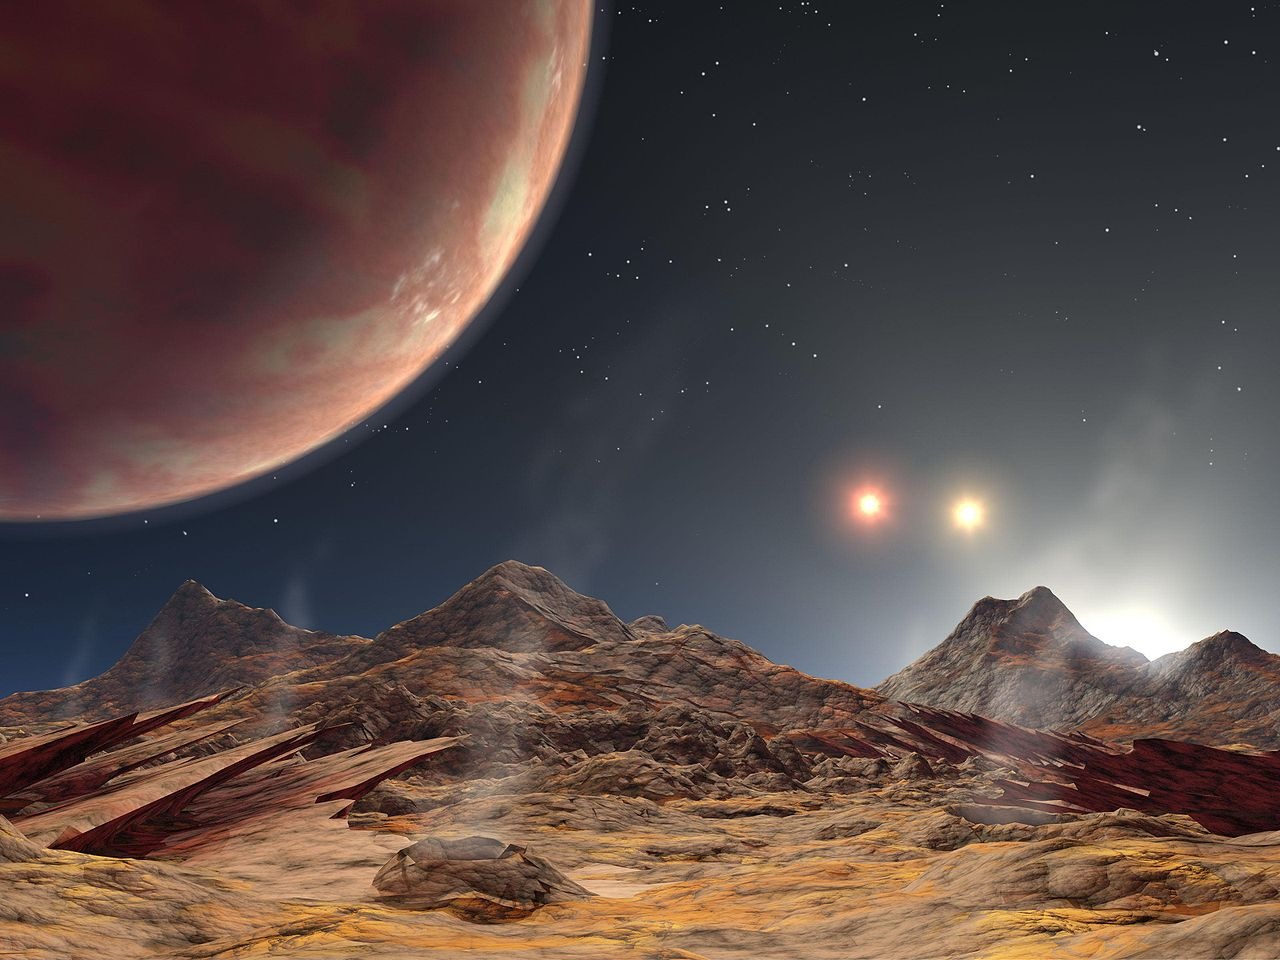
\includegraphics[width=\textwidth]{Pic/Triple-star_sunset.jpg}}


%---------------------------------------------------------------------------------------



%----------------------------------------------------------------------------------------
%	HEADERS
%----------------------------------------------------------------------------------------

\renewcommand{\sectionmark}[1]{\markright{\spacedlowsmallcaps{#1}}} % The header for all pages (oneside) or for even pages (twoside)
%\renewcommand{\subsectionmark}[1]{\markright{\thesubsection~#1}} % Uncomment when using the twoside option - this modifies the header on odd pages
\lehead{\mbox{\llap{\small\thepage\kern1em\color{halfgray} \vline}\color{halfgray}\hspace{0.5em}\rightmark\hfil}} % The header style

\pagestyle{scrheadings} % Enable the headers specified in this block

%----------------------------------------------------------------------------------------
%	TABLE OF CONTENTS & LISTS OF FIGURES AND TABLES
%----------------------------------------------------------------------------------------

\maketitle % Print the title/author/date block
\thispagestyle{empty}
\newpage

{\fontfamily{calligra}\selectfont \begin{huge}
\hspace{1em}
\begin{flushright}
To Lucy
\end{flushright} \end{huge}  }

\newpage
\begin{figure}[h]
\begin{center}
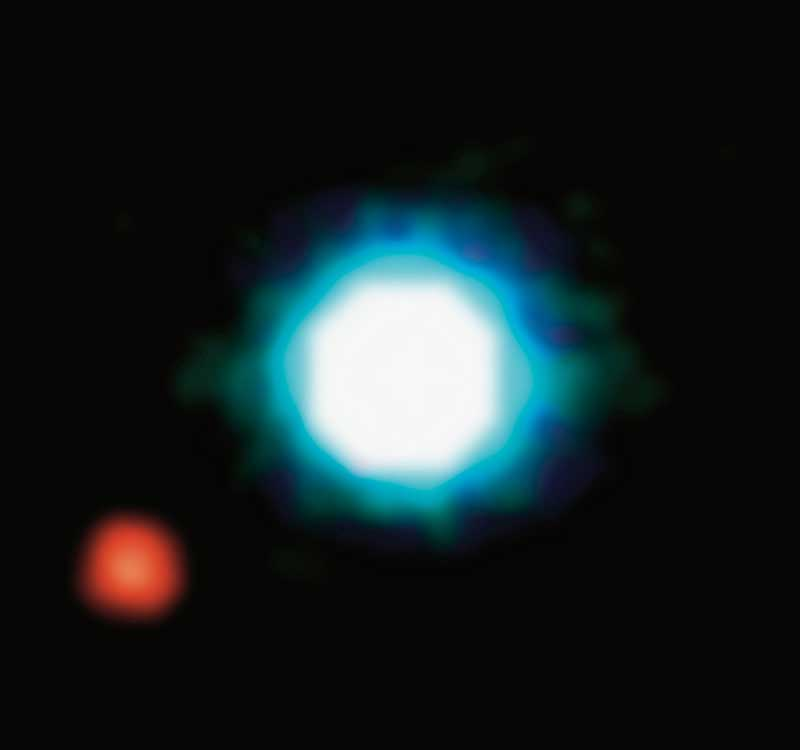
\includegraphics[width=1\textwidth]{Pic/Exoplanet_picture.jpg}
\caption{The 2M1207b exoplanet (red spot) and its host star 2M120 (a brown dwarf) as observed, after three near-infrared exposures (H, K and L wavebands), by the VLT Yepun telescope at the ESO Paranal Observatory. Image taken from \cite{exoplanet_pic}}
\label{Exoplanet_picture}
\end{center}
\end{figure}
\newpage
\setlength\epigraphwidth{.7\textwidth}
\epigraph{ "Listen to me again. Just outside the Galaxy are the Magellanic Clouds, where no human ship has ever penetrated. Beyond that are other small galaxies, and not very far away is the giant Andromeda Galaxy, larger than our own. Beyond that are galaxies by the billions. Our own Galaxy has developed only one species of an intelligence great enough to develop a technological society, but what do we know of the other galaxies? Ours may be atypical. In some of the others-perhaps even in all-there may be many competing intelligent species, struggling with each other, and each incomprehensible to us. Perhaps it is their mutual struggle that preoccupies them, but what if, in some galaxy, one species gains domination over the rest and then has time to consider the possibility of penetrating other galaxies" \newline (I.Asimov, Foundation and Earth)
}



\newpage


%----------------------------------------------------------------------------------------
%	ABSTRACT
%----------------------------------------------------------------------------------------

\section*{Abstract} % This section will not appear in the table of contents due to the star (\section*)
Among the different tools that are considered by scholars to challenge the physical science issues, the statistical learning techniques seems to provide a promising approach to challenge them \cite{carleo2019machine}. This approach can be used to tackle, one of the oldest problem of physical sciences:  the habitability of exoplanets and the possibility of the presence of life on them \cite{seager2013exoplanet}. This approach was previously used by scholars \cite{armstrong2020exoplanet,saha2018machine}: here a group of statistical learning techniques (Decision Tree, Random Forest, Support-vector machines, logistic classification, Linear and Quadratic Discriminant Analysis) were applied and compared to a selected set of 500 exoplanets. The performances of the different methods were also compared using the confusion matrix, the ROC curve and the $/phi$ factor: it was pointed out that the Random forest algorithm provides the best forecasts, followed by the decision tree and the quadratic discriminant analysis. 

\nocite{*}
\setcounter{tocdepth}{2} % Set the depth of the table of contents to show sections and subsections only

\tableofcontents % Print the table of contents

%\listoffigures % Print the list of figures

%\listoftables % Print the list of tables


\newpage % Start the article content on the second page, remove this if you have a longer abstract that goes onto the second page

\section{Introduction}
The possibility of other forms of life on other planets represented an issue that involved scientists as well as philosophers for different millennia of documented human history \cite{papagiannis1985historical}. During the XX century, due to the technological progress, such question moved from a pure speculative approach, as it was previously for Lucretius, Muhammad al-Baqir or Iordanus Brunus, to a more quantitative and scientific method. Furthermore, it is interesting to point out that this research was undertaken when the exploration of the Earth was almost completed \cite{fleming2001barrow}. The exploration of space, and the investigation of other planets was largely boosted by the use of telescopes that measure the radiation also outside the visible spectrum and later with the space telescopes such as the NASA's Kepler. Finally the use of the space probes allowed a closer exploration of planets as wells of moons of solar system \cite{space_probes}. 
Only rocky planets are considered habitable \footnote{In principle also moons have to be considered, however for sake of simplicity here we take into account only planets}, so gaseous ones such as Jupiter or Saturn have to be considered not habitable (see Fig. \ref{exoplanet_populations} and \ref{PT_Confirmed}); second, as requested by all form of life in the Earth, an habitable planet requires that liquid water can be present \cite{seager2013exoplanet,mckay2014requirements,rothschild2001life} \footnote{Astrobiologist scholars also proposed that other form of life can come up without liquid water (see for instance \cite{rahm2016polymorphism}) however, for simplicity, here only planets that allows liquid water are considered habitable}. This feature is given, at first glance, by the radiation intensity $I$ that is bounded to the luminosity ($L$) produced by the star that host the planet and the respective distance $R$. Indeed by approximating a star as a point or a perfect sphere, a radiation with a spherical symmetry is produced; therefore the integral that gives the luminosity $L$: 
\begin{equation}
L=\int \textbf{I}\cdot \textit{d\textbf{A}}
\end{equation}
can be simplified as 
\begin{equation}
L= I \cdot A_{surf}=I\cdot4\pi R^{2}
\end{equation}
and so  \footnote{Further details about this solution and the formalism by which it is obtained from the Maxwell equations can be found in Ref. \cite{feynman}.}
\begin{equation}
 I =\dfrac{L}{4\pi R^{2}}
\label{Flux}
\end{equation}
The latter is called stellar flux. On this basis one can derive the planetary equilibrium temperature starting from the balance equation that equals the flux absorbed by the planet with the emitted one \cite{catling2017atmospheric}: 
\begin{equation}
F_{abs}=F_{emit}
\end{equation}
however since part of incident flux is reflected according to the planet Albedo A, the previous equation can be rewritten in the following way \cite{catling2017atmospheric}:
\begin{equation}
(1-A_{B})F_{solar}=F_{emit}
\end{equation}
furthermore, since only a half hemisphere of a planet can absorb the flux emitted by the half of the star that emits it, we have \cite{catling2017atmospheric}:
\begin{equation}
F_{solar}=\dfrac{I_{0}}{4}
\end{equation}
where I$_{0}$ is the incident radiation on the planet (in this case a scalar). Then plugging the Stefan–Boltzmann law for the radiation of a black-body we obtain \cite{catling2017atmospheric}: 
\begin{equation}
\left(1-A_{B}\right)\dfrac{I_{0}}{4}=\sigma T^{4}_{eq}
\end{equation}
Where $\sigma$ is a constant. Thus the planetary equilibrium temperature will be \cite{catling2017atmospheric}:
\begin{equation}
T_{eq}=\left(\dfrac{I_{0}\left(1-A_{B}\right)}{4\sigma}\right)
\end{equation}
Finally if we plug in the following relation the Eq. \ref{Flux} we obtain \cite{catling2017atmospheric}:
\begin{equation}
T_{eq}=\left(\dfrac{L\left(1-A_{B}\right)}{16\sigma\pi R^{2}}\right)^{\dfrac{1}{4}}
\end{equation}
that can be cast as function of stellar temperature  T$_{star}$ and its radius R$_{s}$ \cite{catling2017atmospheric}:
\begin{equation}
T_{eq}=T_{star}\sqrt{R_{s}/2R}\left(1-A\right)^{0.25}
\end{equation}
Such relation establishes an interval for the distance $R$ where the stellar radiation, here given in function of L or $T_{star}$, is not too hot forcing water in the gas phase, and not to low so that only the solid state phase is allowed. In the literature this interval is usually called habitable-zone. \cite{kasting1993habitable}. However this represents an over-simplified model since no atmospheric effect (except for the albedo) is taken in to account: indeed the surface temperature is also influenced by the greenhouse gases that allows to the host radiation to enter inside the planet but limits its escape \cite{seager2013exoplanet,forget2014possible}. Basically, as explained in figure \ref{Greenhouse-effect-t2},  such phenomena is given by the greenhouse molecules, such as CO$_{2}$, vapour, CH$_{4}$, that are excited by the infra-red radiation produced by the planet. Since these remit the energy gained in all directions, the overall heat that is lost by the planet through infra-red radiation is reduced, as showed in Fig. \ref{BlackBody_greenhouse} \cite{pierrehumbert2011infrared}, thus the surface temperature is increased. It is worth nothing that, in principle, the greenhouse effect does not reduce the habitability: on the contrary it allows to the planet to keep part of the heat received from the host star. On the other side, if the concentration of the greenhouse gases is too high, and therefore the surface temperature abruptly increases, the planetary homoeostasis  \cite{lovelock1974atmospheric,lovelock1982life,caldeira1992life} breaks and the water that is present on the planet escapes from it; this was probably the fate of Venus that lost its oceans \cite{way2016venus,luger2015extreme,seager2013exoplanet}. The conventional habitable zone can be extended if, for instance, we take into account the fact that more massive planets are able to bind the H$_{2}$ (a greenhouse gas see Fig \ref{Planets_habitability_Seager}); therefore also the mass of a planet, in principle should be considered as a factor for its habitability. Scholars \cite{tackley2012habitable} also focused on the tectonic phenomena that allows the recycling of atmospheric gases and produces a negative feedback for surface temperature \cite{walker1981negative}: this feature, at a first glance, is largely influenced by the presence of water \cite{korenaga2010likelihood,o2007geological} and weakly by the planet radius \cite{o2007geological} and mass \cite{korenaga2010likelihood}\footnote{The features reported here, such as the stellar luminosity, represent what we can observe now from the planets and stars: since the speed of light is finite ($3\cdot10^{8}$ m/s ) and many stellar systems are vary far away (for instance 582 light years for Kepler-186) such features describe the planets and stars as these were also centuries ago: therefore the habitability refers to the moment when the light signal was broadcast and not to the present situation.} .  
  

\begin{figure}[h]
\begin{center}
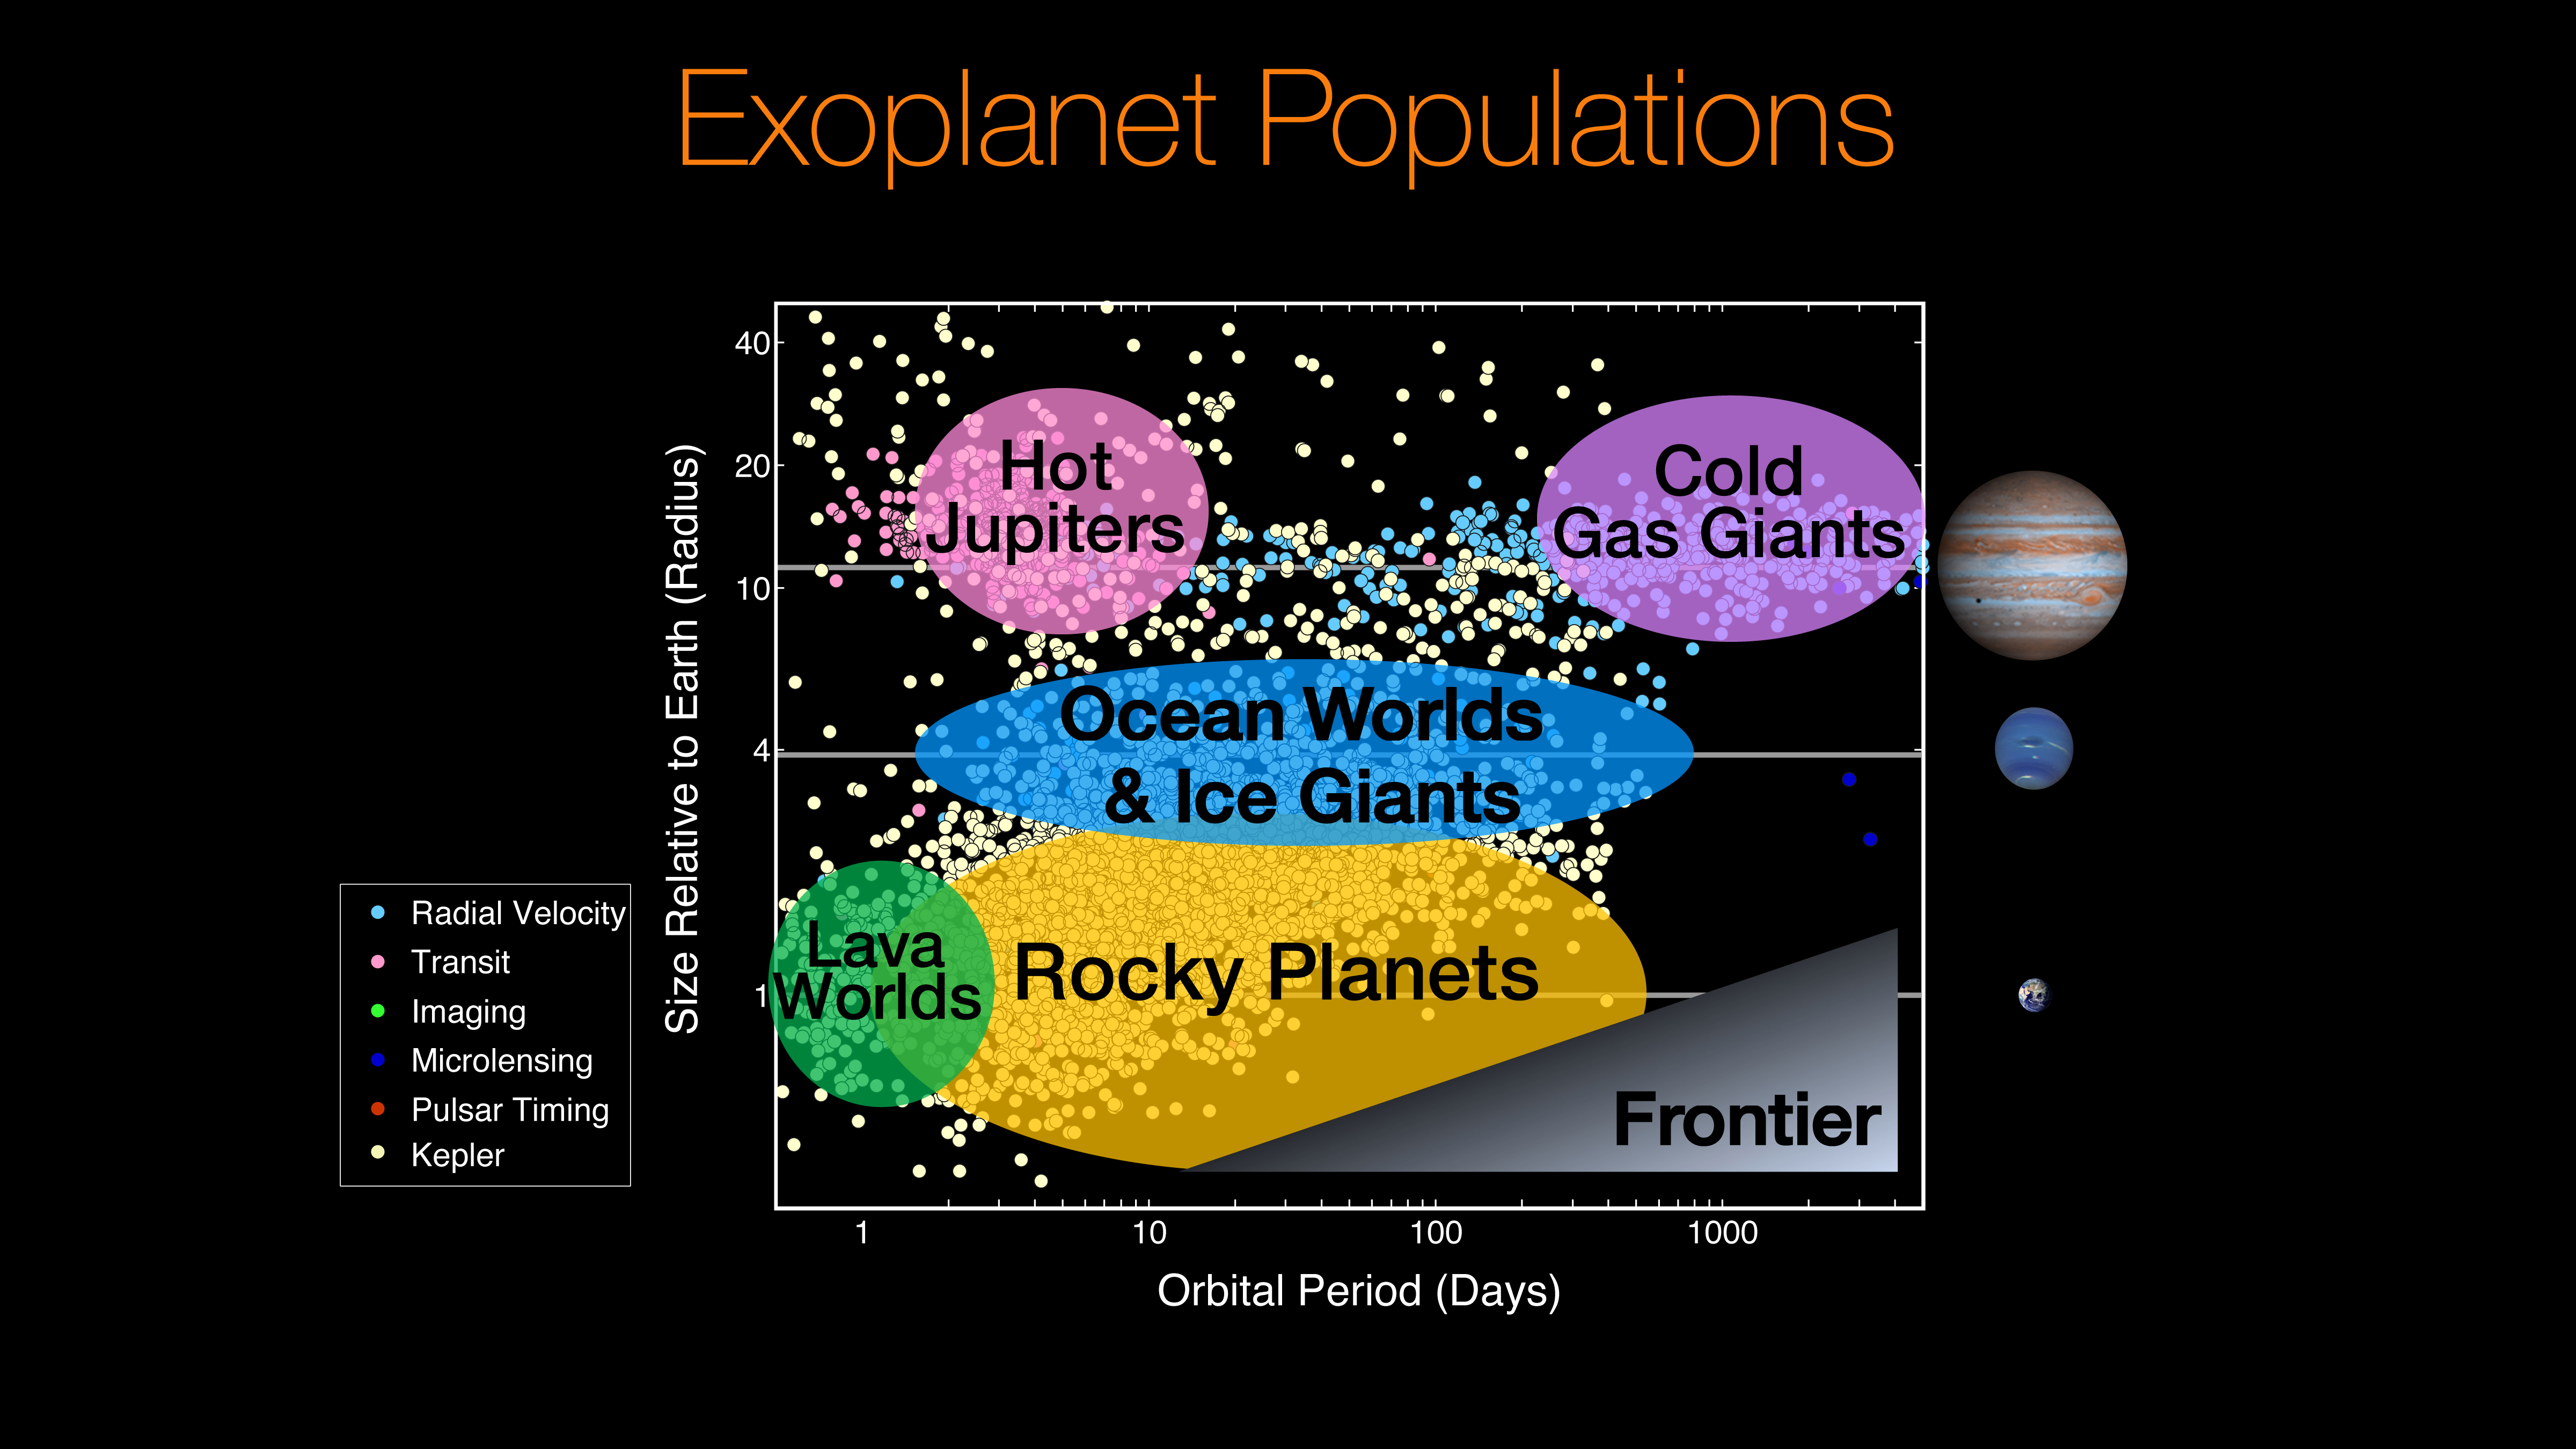
\includegraphics[width=1\textwidth]{Pic/press-web25_exoplanet_populations.jpg}
\caption{A NASA plot about the possible type of exoplanets given their orbital period and size. Image taken from \cite{exoplanet_populations}}
\label{exoplanet_populations}
\end{center}
\end{figure}

\begin{figure}[h]
\begin{center}
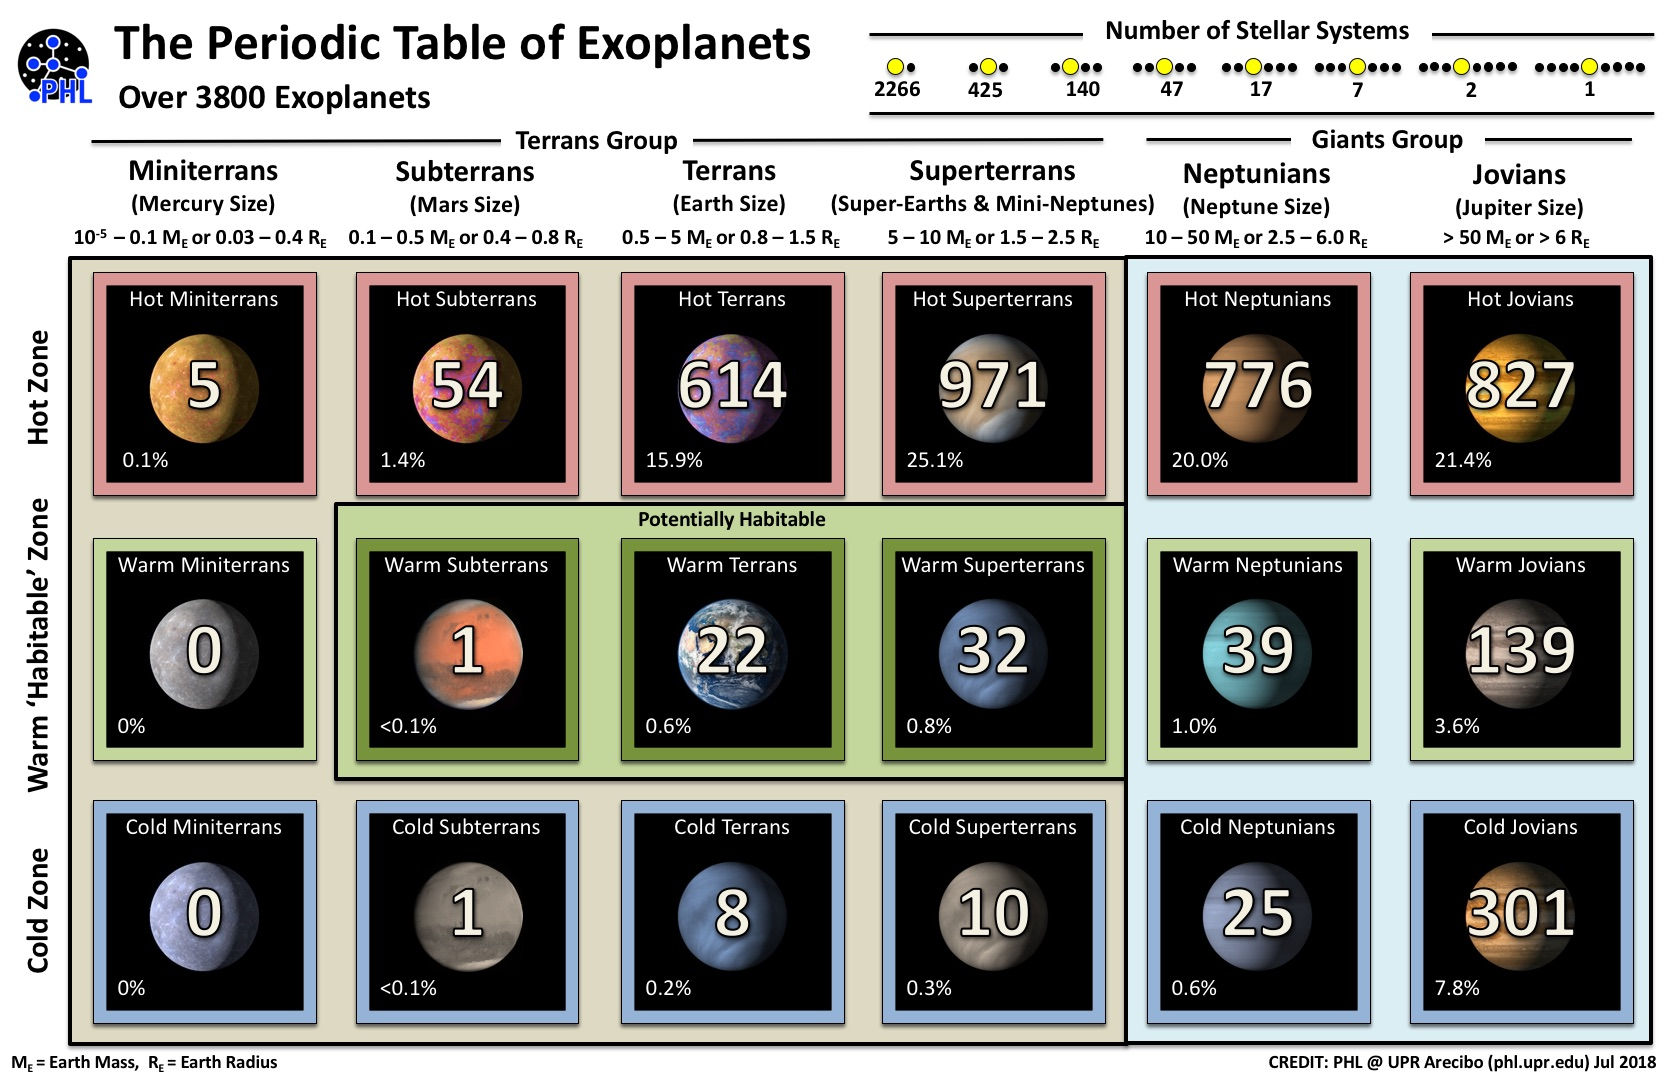
\includegraphics[width=1\textwidth]{Pic/PT_Confirmed.jpg}
\caption{PHL @ UPR Arecibo classification of the different exoplanets. Image taken from \cite{exoplanets-catalog}}
\label{PT_Confirmed}
\end{center}
\end{figure}


\begin{figure}[h]
\begin{center}
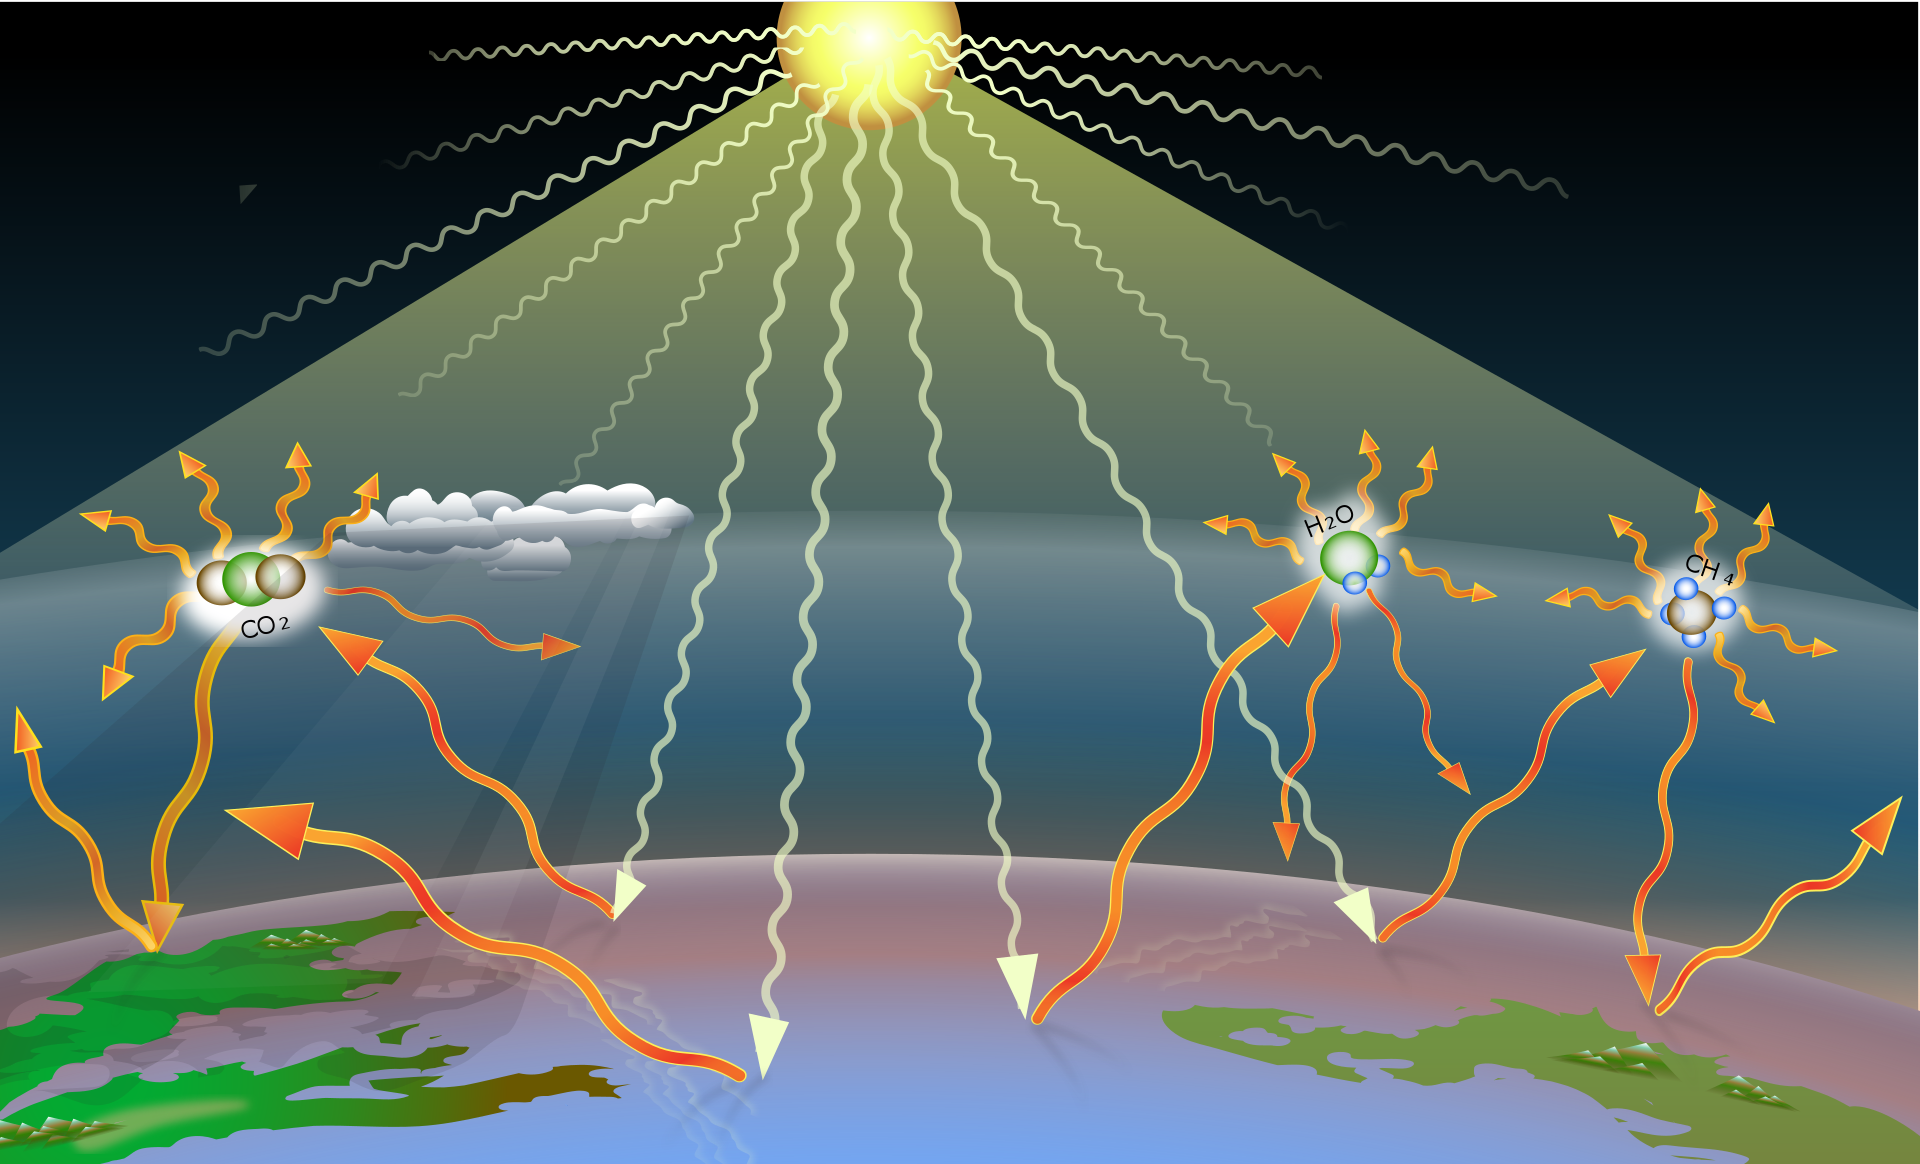
\includegraphics[width=1\textwidth]{Pic/Greenhouse-effect-t2.png}
\caption{The greenhouse effect: the radiation of the host star is captured by the planet and than remitted: this process is limited by the greenhouse molecules of the athomosphere that absorb and re-emit the radiation in all directions. Image taken from \cite{Greenhouse-effect-t2}}
\label{Greenhouse-effect-t2}
\end{center}
\end{figure}

\begin{figure}[h]
\begin{center}
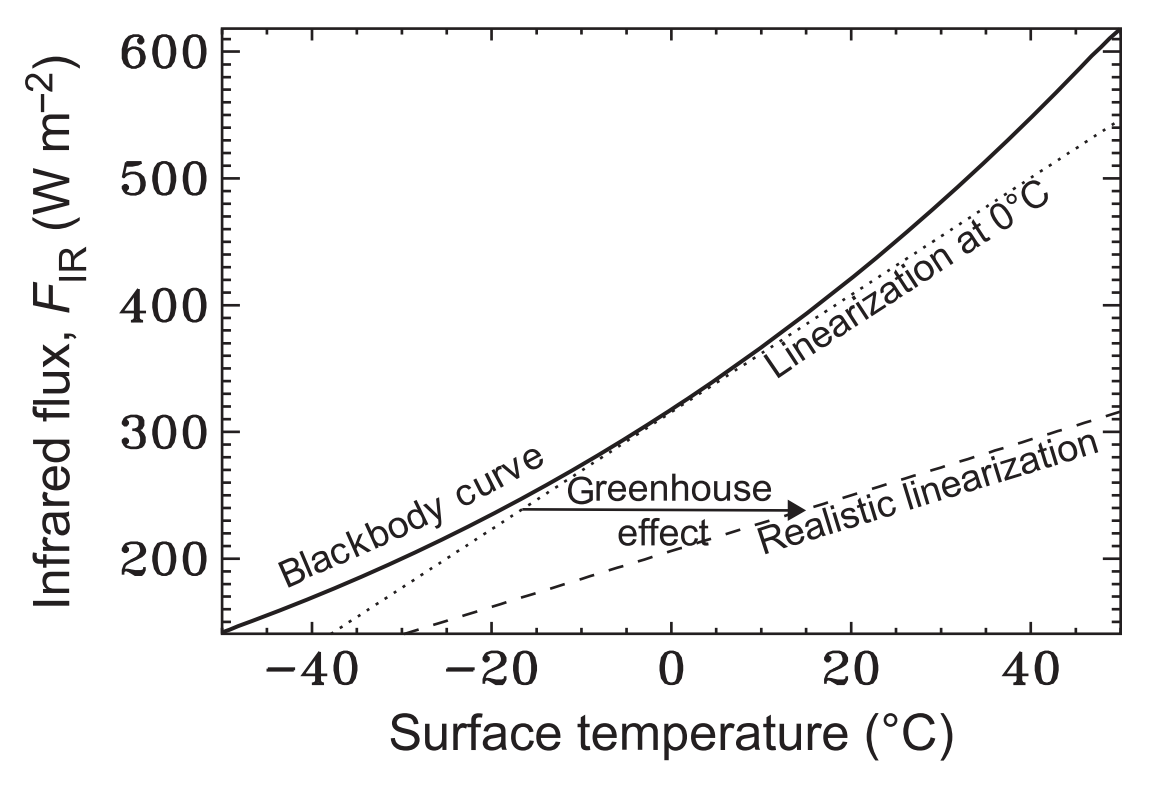
\includegraphics[width=1\textwidth]{Pic/BlackBody_greenhouse.png}
\caption{The infrared radiation emitted if the explanet is a perfect blackbody and if the greenhouse effect is considered. Image taken from \cite{catling2017atmospheric}}
\label{BlackBody_greenhouse}
\end{center}
\end{figure}

\begin{figure}[h]
\begin{center}
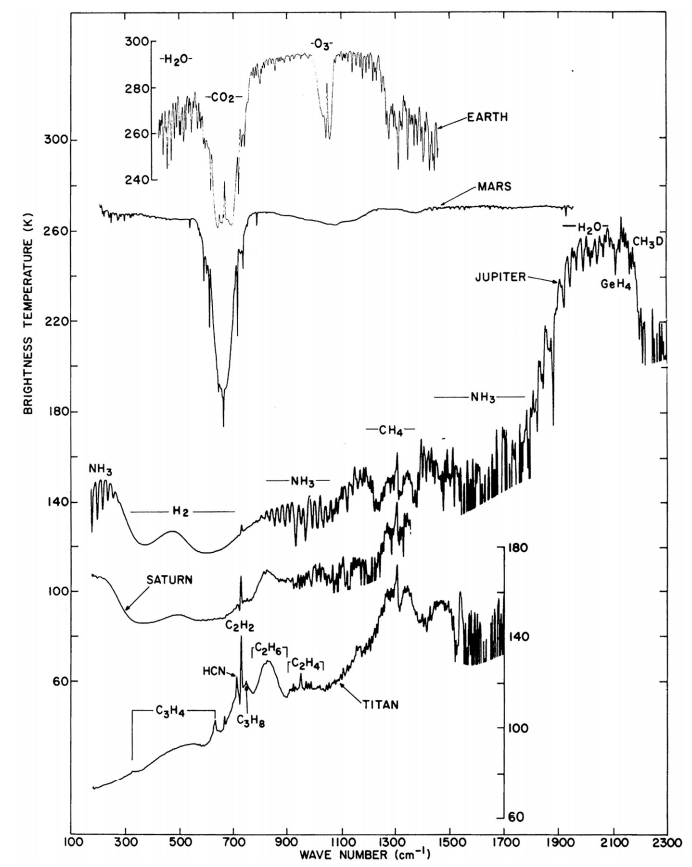
\includegraphics[width=1\textwidth]{Pic/Absorption_gas.png}
\caption{The spectra of a selected set of planets/moons. The peaks that fingerprint the presence of atmospheric gases are also reported. Image taken from \cite{catling2017atmospheric}}
\label{BlackBody_greenhouse_2}
\end{center}
\end{figure}

\begin{figure}[h]
\begin{center}
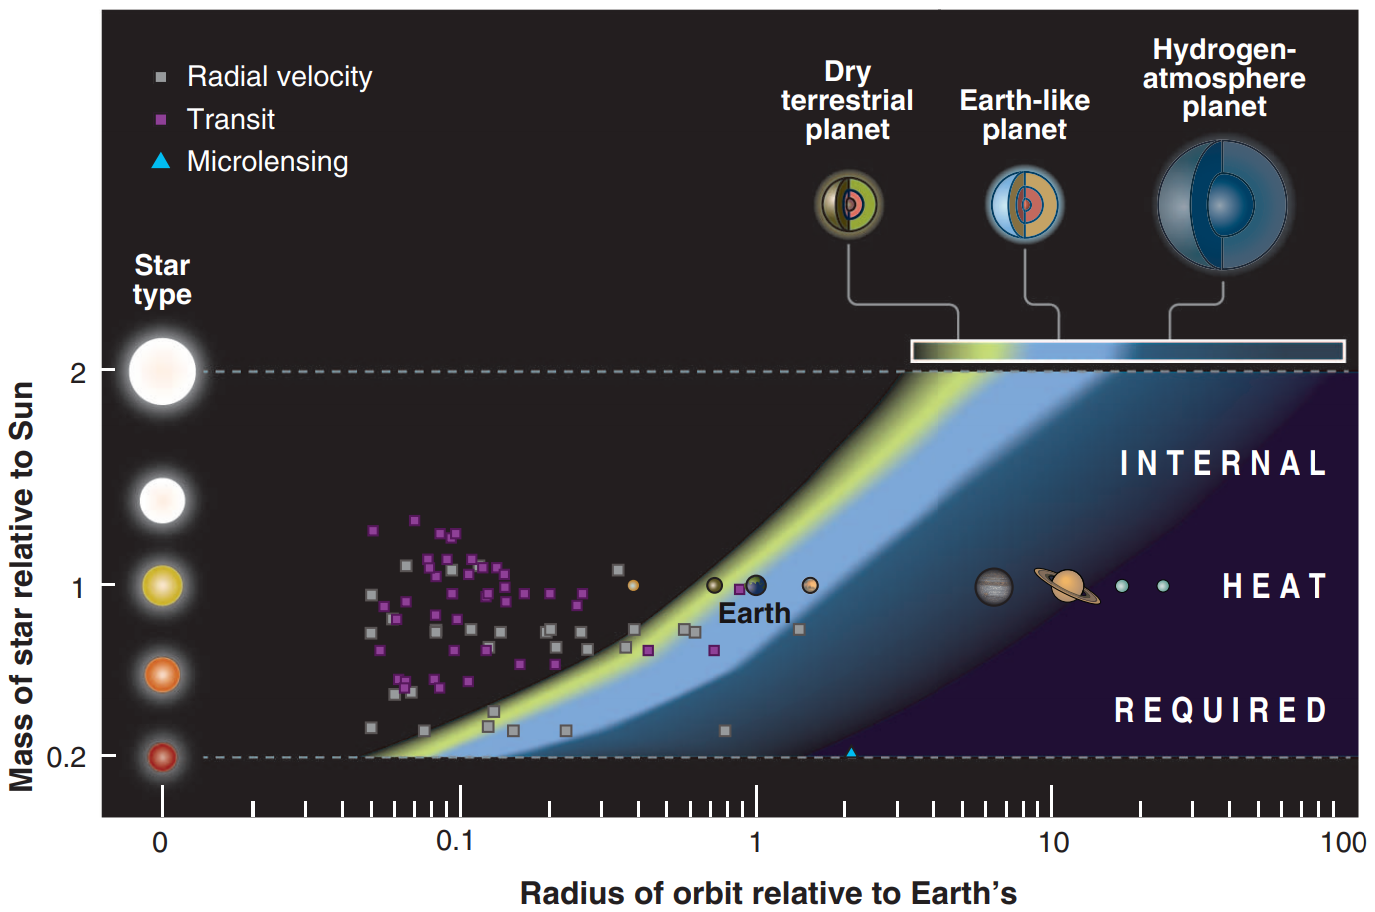
\includegraphics[width=1\textwidth]{Pic/Planets_habitability_Seager.png}
\caption{Seager representation of planet habitability as function of star type (that determinates the stellar activity) planet distance and its atmosphere: the light blue is the conventional habitable zone, while the dark blue and green one represent the extension of it due to the peculiarity of the planets. Image taken from \cite{seager2013exoplanet}}
\label{Planets_habitability_Seager}
\end{center}
\end{figure}


\clearpage

\section{Data Description}

The planet dataset was taken from the \textit{Planetary Habitability Laboratory @ UPR Arecibo} \cite{planet_dataset} website. Since the habitable planets, considering also the optimistic region, were  55 out of 3500, a reduction of the non-habitable planets to 445 (extracted randomly\footnote{The overall results exposed here were double checked with two extractions. The extraction used in this work was saved in the file Planet\_ dataset.rda }) was undertaken in order to make the habitable planets a significant portion of the overall set. As reported in table \ref{features_table}, among the different features that were provided by PHL, a restricted set was considered: such operation was performed in order to avoid features whose causal effect on the habitability (where it was present) do not require very complex models/explanation \footnote{But may be considered as a future outlook}. For all the exoplanets considered in this work the features reported in the table \ref{features_table} were well-defined. 
 

\begin{table}[]
\caption{A selected features of the exoplanets dataset provided by PHL @ UPR Arecibo \cite{planet_dataset} accompanied by their measure unit }
\begin{tabular}{@{}lll@{}}
\toprule
Variable name                                                                & Abbreviation & Description/Comments                                                                                      \\ \midrule
Planet name                                                                  & P\_NAME      & \begin{tabular}[c]{@{}l@{}}The planet name according to \\ the international convention\end{tabular}      \\ \midrule
Planet Period                                                                & P\_P         & The planet period (days)                                                                                  \\ \midrule
Stellar temperature                                                          & S\_T         & \begin{tabular}[c]{@{}l@{}}The star effective temperature\\ (K)\end{tabular}                              \\ \midrule
Planet distance                                                              & P\_D         & \begin{tabular}[c]{@{}l@{}}Mean distance between the planet \\ and the host star (AU)\end{tabular}        \\ \midrule
Planet Periastron                                                            & P\_PN         & \begin{tabular}[c]{@{}l@{}}The minimum distance between \\ the planet and the host star (AU)\end{tabular} \\ \midrule
Planet apastron                                                              & P\_A         & \begin{tabular}[c]{@{}l@{}}The maximum distance between \\ the planet and host star (AU)\end{tabular}     \\ \midrule
\begin{tabular}[c]{@{}l@{}}Planet effective \\ thermal distance\end{tabular} & P\_D\_E      & (AU)                                                                                                      \\ \midrule
\begin{tabular}[c]{@{}l@{}}Planet mean stellar\\ flux\end{tabular}           & P\_F         & (earth units)                                                                                             \\ \midrule
\begin{tabular}[c]{@{}l@{}}Planet equilibrium \\ temperature\end{tabular}    & P\_T\_E      & An albedo of 0.3 is considered (K)                                                                        \\ \midrule
Star radius estimated                                                        & S\_R\_E      & (solar units)                                                                                             \\ \midrule
Star luminosity                                                              & S\_L         & (solar units)                                                                                             \\ \midrule
Planet Habitability                                                          & P\_H         & Boolean                                                                                      \\ \midrule
\begin{tabular}[c]{@{}l@{}}Estimated planet \\ radius\end{tabular}           & P\_R         & (earth units)                                                                                             \\ \midrule
\begin{tabular}[c]{@{}l@{}}Estimated planet\\ mass\end{tabular}              & P\_M         & (earth units)                                                                                             \\ \midrule
Star Spectral Type                                                           & S\_S\_T      & \begin{tabular}[c]{@{}l@{}}The star spectral type according\\ to the diagram in Fig. \ref{H_R_diagram} \end{tabular}         \\ \bottomrule
\end{tabular}
\label{features_table}
\end{table}

\begin{figure}[h]
\begin{center}
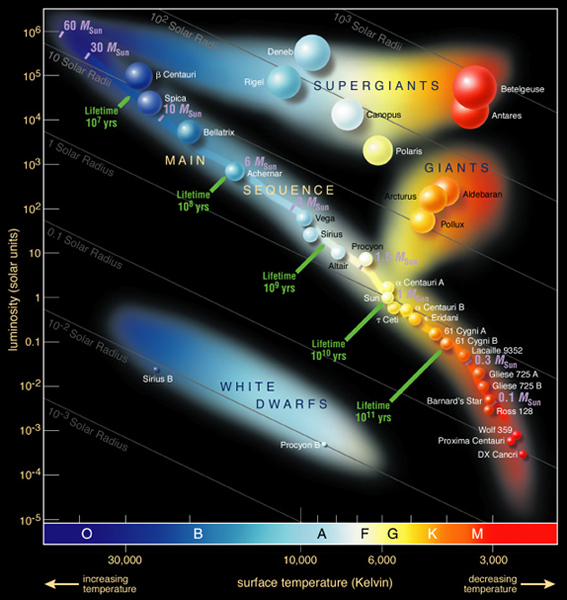
\includegraphics[width=0.9\textwidth]{Pic/S_T_T_explanation.png}
\caption{The Hertzsprung–Russell diagram (H-R): the phases that occurs during the lifetime of a star are placed on a plot that involves the surface temperature (and so the spectral type) vs the star luminosity .   Image taken from \cite{HR_diagram}}
\label{H_R_diagram}
\end{center}
\end{figure}


\clearpage

\section{Theoretical Background}

In this section the theoretical background of the methods used in this work are rapidly summarized following the James at al. approach \cite{james2013introduction}; these are: the decision tree, the random forest, the support vector classifier (for which a dimensionality reduction via the principal component analysis (PCA) was performed), the logistic regression and the linear and the quadratic discriminant analysis. 
Before reviewing them, it is useful to recap the basic concepts on which the supervised learning is founded. \newline\newline Lets consider a process, or more precisely a dynamical system,  where there is a set of variables \textbf{X} that represent the different initial conditions, called inputs, and a set of respective final conditions, called outputs \textbf{Y}. Moreover lets suppose that the, at a first inspection the machinery of the dynamical system it is inaccessible (a black-box), however one is still interested to predict some unknown output given some known input. Formally we are intended to approximate the dynamical system with the following relation \cite{james2013introduction}: 
\begin{equation}
\textbf{Y}=f(\textbf{X})+\epsilon
\end{equation}
where the $\epsilon$ represents the irreducible error term introduced by the approximation of the dynamical system (basically we will never know the exact laws that govern the phenomena, and also if these were known we will always have an error term due to finite precision by which we approximate the initial conditions \cite{prigogine2018order,prigogine1997end,petrosky1996liouville}\footnote{The difference between the \textit{true} and the predicted orbits and their divergence was investigated by Lyapunov \cite{liapounoff1907probleme}: basically the two trajectories diverges in time following the following relation: $ \lvert \delta\textbf{Z} \rvert \approx e^{\lambda t} \lvert \delta\textbf{Z}_{0} \rvert $ where  $\lambda$ the Lyapunov coefficient, $\lvert \delta\textbf{Z}_{0} \rvert$ and  $\lvert \delta\textbf{Z} \rvert $ respectively  the initial and final differences between the trajectories, with respect to the time evolution $t$}  ). Basically the aim of the statical learning theory is to estimate, with different methods, the response function $f$ \footnote{A useful approximation, especially in physics, of the response function is the linear response function $\chi(t-t')$ for an input h(t), where t represent the time, and an output x(t) is defined as $x(t)=\int_{-\infty}^{t}dt'\chi(t-t')h(t')+\epsilon$, where $\epsilon$ is due to the fact that we approximated the response function as a linear one. The linear response function is closely related to the Green function that plays a crucial role in the modern physics (for instance in the quantum field theory \cite{kubo1957statistical,zee2010quantum})}. It worth nothing that a very interesting application of this approach was performed by Claude Shannon \cite{shannon2001mathematical,mackay2003information} when he founded the information theory: in this case, as shown in Fig \ref{Noisy_channel} we can fix the input \textbf{X} as the signal produced and the output \textbf{Y} as the signal received, since no perfect channel is available the output signal will be distorted, thus the idea is how to infer from the output signal the input one.
\begin{figure}[h]
\begin{center}
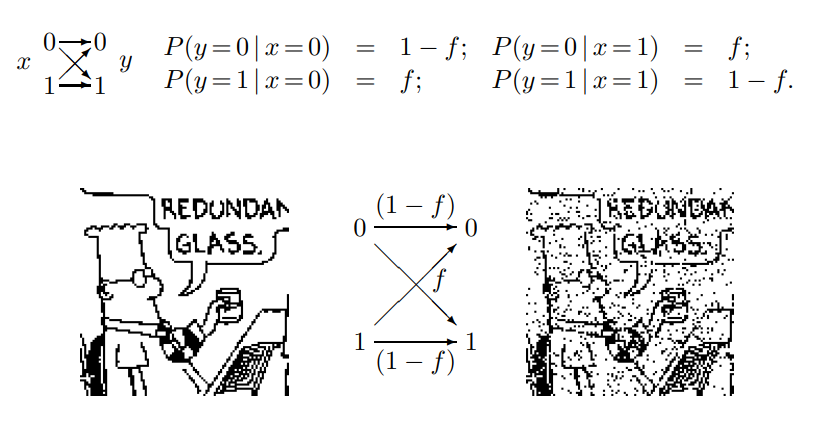
\includegraphics[width=0.9\textwidth]{Pic/Noisy_channel.png}
\caption{A sequence of binary data transmitted over a binary symmetric channel with noise equal to $f=0.1$   Image taken from \cite{mackay2003information}}
\label{Noisy_channel}
\end{center}
\end{figure}
Basically the approaches by which the problem of finding (inference) or forecasting (prediction) the behaviour of the response function are two: the parametric methods and the non-parametric. Parametric methods perform firstly an approximation on the response function (e.g. it is linear), then use a part of the known input and output to estimate the parameters of the model by which the response function was approximated and finally the reaming values of input and output are used to validate the model; here the main risk is to introduce too many parameters that fits not only the response function but also the noise, thus when the input will be changed (with the test input/output) the error will abruptly increase: such behaviour is know as over-fitting. \footnote{Overfitting can be quickly described with an Enrico Fermi answer to Freeman Dyson: "How many arbitrary parameters did you use for your calculations?" I thought for a moment about our cut-off procedures and said, "Four." He said, "I remember my friend Johnny von Neumann used to say, with four parameters I can fit an elephant, and with five I can make him wiggle his trunk." \cite{dyson}}. On the other side, one can make no assumptions on the form of the response function (and so the model is more flexible) and try to estimate an f that is close as possible to the data point: these are the non-parametric methods; note that also in this case the over-fitting is possible. 


\clearpage

\subsection{Decision tree}

The basic idea of this approach is to divide the space of the predictor \textbf{X} in a set of a different subspaces, and then imposing that predictors that are in the same subspace have the same output value. Thus the problem is shifted to the creation of subspaces and their shape. Concerning the shape the most easy approach is to consider rectangles or, for higher dimensions, boxes; on the other side the creation of them can be performed by a top down approach where each box is divided in two sub-box, via the minimization of the RSS: given a predictor $X_{j}$ the cut-points s of boxes j are chosen so that, given \cite{james2013introduction}:   
\begin{equation}
R_{1}(j,s)= \{X | X_{j} < s \} \quad R_{2}(j,s)= \{X | X_{j} > s \}
\end{equation}
they minimize the following equation \cite{james2013introduction}: 
\begin{equation}
\sum_{i: x_{i} \in  R_{1}(j,s)}(y_{i}-\hat{y}_{R_{1}})^{2}+\sum_{i: x_{i} \in  R_{2}(j,s)}(y_{i}-\hat{y}_{R_{2}})^{2}
\end{equation}
where $\hat{y}_{R_{1}}$ represent the mean response for the training observation in $R_{1}(j,s)$. This splitting is performed recursively until each box contains no more than a fixed quantity of points. Finally the answer of the points contained in the same box will be identical. In order to avoid over-fitting one can consider to limit the splitting when the pay-off between the generation of a new sub-tree and the over-fitting threat is not convenient;formally this can be done by using the following expression \cite{james2013introduction}: 
\begin{equation}
\sum_{m=1}^{|T|}\sum_{x_{i}\in R_{m}}(y_{i}-\hat{y}_{R_{m}})^{2}+\alpha|T|
\end{equation}
where $\alpha$ represent the penalising factor when a new sub-tree is generated and |T| the number of terminal nodes of tree T. Such approach is called pruning. Finally if the output is class (as in this work: habitable or not) the RSS approach has to be replaced with the Gini index \footnote{This index was proposed by Corrado Gini to measure the inequality distribution of wealth in a country \cite{gini1912variabilita}}
\begin{equation}
G=\sum_{k=1}^{K}\hat{p}_{mk}(1-\hat{p}_{mk})
\end{equation}
or by the entropy \footnote{The entropy, introduced firstly by Rudolf Clausius and later developed by  Ludwig Boltzmann and Josiah Willard Gibbs, is concept that was initially introduced in physics: it was used to quantify the spontaneity of a transformation (\textgreek{entropía}-entropía, "a turning towards"). This because all the law of classical mechanics are symmetric with respect to the inversion of time and so the physical phenomena such as the diffusion of a gas (and not its spontaneous accumulation) cannot be explained only with them. Note that this issue, that was first formalized by \cite{loschmidt1876grosse,wu1975boltzmann}  was solved only recently with the fluctuation theorem \cite{evans1993probability,wang2002experimental}. The form used here is basically the scaled Gibbs expression (in which the Boltzmann constant $k_{b}$ was set to 1)}
\begin{equation}
D=-\sum_{k=1}^{K}\hat{p}_{mk}log\hat{p}_{mk}
\end{equation}
these indices, as evaluated here, measure the degree of purity of a node: if all the values are close to zero or one, their values will be close to 0. The decision tree approach provide therefore a results that is easily interpretable, drawable and communicable; on the other side among the statistical learning tools is not the one that provide the highest predictive accuracy and stability. 


\paragraph{Bagging}

In order to make the decision tree result more independent from the training dataset chosen (the over-fitting problem described before) one can consider to generate further training sets, via bootstrap method, in order to reduce the variance of the model. Thus the final model will be given by \cite{james2013introduction}: 
\begin{equation}
\hat{f}_{bag}\left(x\right)=\dfrac{1}{B}\sum_{b=1}^{B}\hat{f}^{*b}\left(x\right)
\end{equation}
Where $B$ is the overall number of training sets generated via the bootstrap and $\hat{f}^{*b}$ the statistical model obtained from the $b^{th}$ training set. If a classification problem is undertaken, the class predicted will given by the one that is most common among the B predictions (majority rule).


\paragraph{Random forest} 
The random forest technique, firstly introduced in 1995 \cite{ho1995random}, represent a further improvement of the decision tree after bagging: in this case, for each split, a random subset m of the full predictor set p is used. Such procedure is perform in order to avoid that the decision tree generated with the bootstrap are too similar due to the fact that there only few predictor that dominates the others, otherwise the reduction of variance due to the bagging is not so efficient since the bagged trees are correlated. The full random forest algorithm can be explained with the following analogy \cite{rand_for_exp}: lets consider a man, Carlo,  that would like to made a trip and, for this propose,  he asks to different people a suggestion; these asks to him a set of questions (last trip, sea or mountain, budget etc.) and give to him a final propose. Carlo at least takes a decision by using all the answers. In this example the different peoples are the bagged trees that give an answer basing of a different set of predictors . This algorithm is described in Fig \ref{random-forest-algorithm2}.   
\begin{figure}[h]
\begin{center}
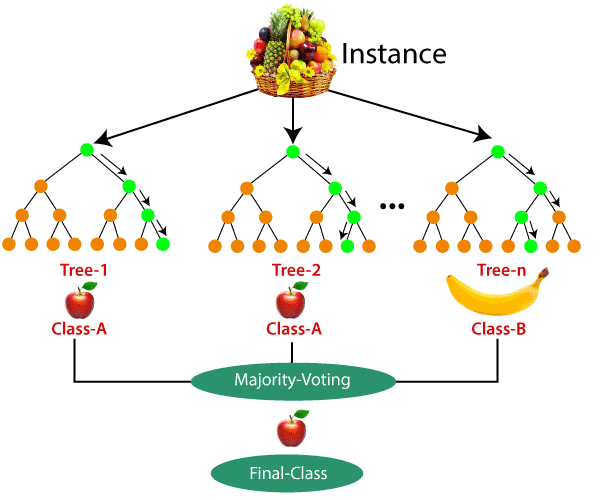
\includegraphics[width=0.9\textwidth]{Pic/random-forest-algorithm2.png}
\caption{A schematic representation of the random forest algorithm. Image taken from \cite{rand_for_fig}}
\label{random-forest-algorithm2}
\end{center}
\end{figure}

\clearpage
\subsection{Support vector machines}
The basic idea of the support vector machines is to consider the input set \textbf{X} ($n\times P$, where n stands for the observations and p for the features) as an ensemble of n-points immersed into a p-dimensional space. Furthermore each point is labelled only in two way \footnote{The approaches described here can be extended to a multiple classes problem as shown in \cite{james2013introduction}, however since in this work only two classes are allowed (habitable or not) this such implementation will not be reviewed}. Thus, with this representation, the classification problem is recast in to a partition of a hyperspace. The simple form by which an hyperspace can be partitioned is an hyperplane \cite{james2013introduction}: 
\begin{equation}
\beta_{0}+\beta_{1}x_{i1}+\beta_{1}x_{i2}+...+\beta_{p}x_{ip} > 0\quad if \quad y_{i}=1
\end{equation}
\begin{equation}
\beta_{0}+\beta_{1}x_{i1}+\beta_{1}x_{i2}+...+\beta_{p}x_{ip} < 0\quad if \quad y_{i}=0
\end{equation}
The problem now is how to choose the hyperplane: this is a first discriminant between the SVM methods, moreover anything guarantee that the boundary is linear and thus a simple hyperplane can be used; this is a second discriminant between the SVM methods. It is worth noting that in principle one can introduce a further dimension, as shown in Fig \ref{Kernel_methods} in order to have a linear hyperplane: this is the idea of the kernel methods\cite{james2013introduction,marsland2015machine}. 
\begin{figure}[h]
\begin{center}
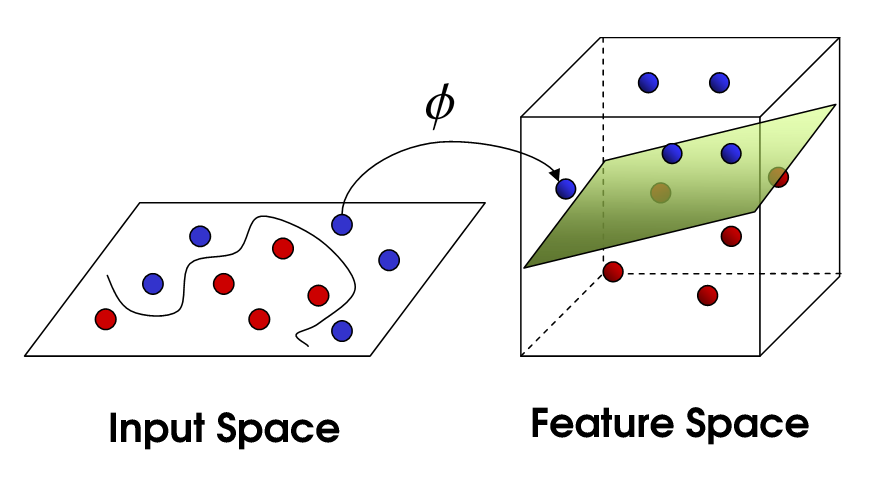
\includegraphics[width=0.9\textwidth]{Pic/kernel_trick.png}
\caption{The trick of the kernel methods: introducing an extra dimension they transform a non-linear boundary in to a linear one. Image taken from \cite{kernel}}
\label{Kernel_methods}
\end{center}
\end{figure}
\paragraph{Maximal margin Classifier}
The maximal margin classifier approach consist in tracing the separating hyperplane so that it has the  farthest minimum distance with respect to the training observation or more formally \cite{james2013introduction}: 
\begin{equation}
\max\limits_{{\beta_{0},\beta_{1}...\beta_{p},M}} M
\end{equation}
\begin{equation}
subject\;to\;\sum_{j=1}^{p}\beta_{j}^{2}=1
\end{equation}
\begin{equation}
y_{i}\left( \beta_{0} + \beta_{1} x_{i1} + \beta_{2} x_{i2}+...+\beta x_{ip}\right)\geq M\quad\forall\; i=1,...,n
\end{equation}
\paragraph{Support vector Classifier}
The maximal margin approach assumes that the separating hyperplane exists, however this is far from be the most common type of classification problem. To overcome to this point the support vector classifier was proposed: in this approach the margin is considered soft allowing some point to be on the wrong side of the margin or on the wrong side of the hyperplane. The tolerance threshold is fixed by a quantity that is called budget $C$, more formally \cite{james2013introduction}:
\begin{equation}
\max\limits_{{\beta_{0},\beta_{1}...\beta_{p},M}} M
\end{equation}
\begin{equation}
subject\;to\;\sum_{j=1}^{p}\beta_{j}^{2}=1
\end{equation}
\begin{equation}
y_{i}\left( \beta_{0} + \beta_{1} x_{i1} + \beta_{2} x_{i2}+...+\beta x_{ip}\right)\geq M\left(1-\epsilon_{i}\right)
\end{equation}
\begin{equation}
\epsilon_{i}\geq 0 \sum_{i=1}^{n}\epsilon_{i}\leq C
\end{equation}
It is worth noting that if the budged is large a low variance will be found but with the toll of high bias; on the other side if the budget is low a low bias will be obtained but with the toll of high variance. Thus the selection of this parameter is crucial.  
\paragraph{Support vector machines}
This is the overall generalization of the method previously described: in particular the idea is to go beyond to the linear boundary. For this purpose the in the general expression \cite{james2013introduction}
\begin{equation}
f(x)=\beta_{0}+\sum_{i\in S}\alpha_{i}K(x,x_{i}) 
\end{equation}
the linear kernel \cite{james2013introduction}
\begin{equation}
K(x_{i},x_{i'})=\sum^{p}_{j=1}x_{ij}x_{i'j}
\end{equation}
is replaced with other kernels \footnote{Such functions are quite close to the correlation functions as defined in statistical mechanics, and then extended in quantum field theory (QFT). In statistical mechanics the correlation functions are defined as \cite{huang1963statistical} $C(r,\tau)= \left\langle s_{1}(\textbf{R},t)\cdot s_{2}(\textbf{R+r},t+\tau)\right\rangle -  \left\langle s_{1}(\textbf{R},t)\cdot s_{2}\right\rangle\left\langle( s_{1}(\textbf{R+r},t+\tau))\right\rangle $ where $s_{1}$ and $s_{2}$ are two random functions, while in QFT these are defined as \cite{zee2010quantum}  $C(x_{1},x_{2},...,x_{n})=\left\langle \phi (x_{1}),\phi(x_{2}),...,\phi(x_{n}) \right\rangle$ where $\phi(x_{n})$ are the field operators. Such analogy is due to the fact that statistical learning and statistical mechanics both face the response functions described before}, as reported in Fig \ref{SVM_kernels} such as the polynomial of degree d \cite{james2013introduction}
\begin{equation}
K(x_{i},x_{i'})=\left(1+\sum_{j=1}^{p}x_{ij}x_{i'j}\right)^{d}
\end{equation}
or perhaps with a radial one \cite{james2013introduction}
\begin{equation}
K(x_{i},x_{i'})=exp\left(-\gamma\sum^{p}_{j=1}\left(x_{ij}-x_{i'j}\right)\right)^{2}
\end{equation}
where $\gamma$ is a positive constant. 
\begin{figure}[h]
\begin{center}
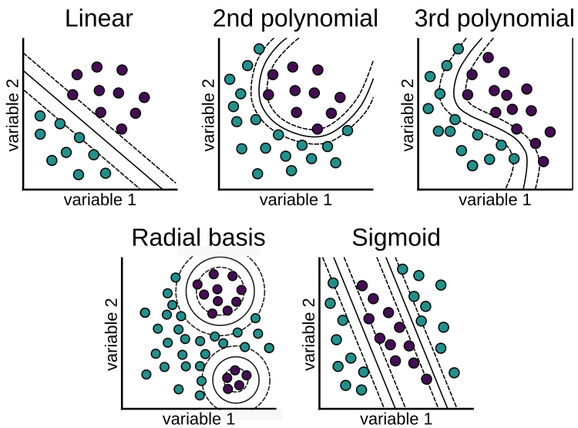
\includegraphics[width=0.9\textwidth]{Pic/Kernels_Type.png}
\caption{A set of possible type of kernels for the SVM. Image taken from \cite{ker_svm}}
\label{SVM_kernels}
\end{center}
\end{figure}
\subsection{Logistic regression}
Beside the methods previously described one may consider to model the relationship between $p(X)=Pr(Y=1|X)$ and $X$ with the logistic function \footnote{The logistic function was originally developed in to a very different context: indeed it was proposed by Pierre Francois Verhulst \cite{verhulst1838correspondance} for the development of a grown population model. Later this function was considered into other fields such as statistical learning}  \cite{james2013introduction}
\begin{equation}
p(X)=\dfrac{e^{\beta_{0}+\beta_{1}X}}{1+e^{\beta_{0}+\beta_{1}X}}
\end{equation}
or, as in this work, a multidimensional set is considered \cite{james2013introduction}
\begin{equation}
p(\textbf{X})=\dfrac{e^{\beta_{0}+\beta_{1}X_{1}+...+\beta_{p}X_{p}}}{1+e^{\beta_{0}+\beta_{1}X_{1}+...+\beta_{p}X_{p}}}
\end{equation}
where the estimation of the parameters $\beta$ is achieved via the maximum likehood method. Such approach is for a binary response, as in our case, but it can be extended to multiple ones.
\subsection{Linear and quadratic vector classifier}
The linear and quadratic classifier are an improvement of the logistic model approach since the logistic one is unstable when the classes are well-separated, moreover these approaches are more stable if $n$ is small. The starting point is the is the Bayes theorem \cite{james2013introduction}:
\begin{equation}
p(Y=k|X=x)=\dfrac{\pi_{k}f_{k}(x)}{\sum_{l=1}^{K}\pi_{l}f_{l}(x)}
\end{equation}
where $f(x)$ is the density function of X from an observation from k$^{th}$ class  $f_{k}\coloneqq Pr(X=x|Y=k)$ and $\pi_{k}$ the prior probability that a random observation come from the k$^{th}$ class \cite{james2013introduction}. 

\subparagraph{Linear discriminant analysis}
Here the density $f(x)$ is assumed to be a multivariate gaussian distribution\cite{james2013introduction}: 
\begin{equation}
f(\textbf{x})=\dfrac{1}{\left(2 \pi\right)^{p/2}\lvert \boldsymbol {\Sigma}\rvert^{-1/2} }exp \left(-\frac{1}{2}\left(\textbf{x}-\boldsymbol{\mu}\right)^{T}\boldsymbol {\Sigma}^{-1}\left(\textbf{x}-\boldsymbol{\mu}\right)\right)
\end{equation}
While the covariance matrix $\boldsymbol {\Sigma}$ is common for all classes while $\boldsymbol{\mu}$ is different for each of them. Thus, by some manipulation one obtains that the Bayes classifier put an observation $X=\textbf{x}$ for which \cite{james2013introduction}:
\begin{equation}
\delta(\textbf{x})=x^{T} \boldsymbol {\Sigma}^{-1} \mu_{k}-\frac{1}{2}\mu^{T}_{k}\boldsymbol {\Sigma}^{-1}\mu_{k}+log\pi_{k}
\end{equation}
is largest. Note the linearity of the expression with respect to the \textbf{x} vector, that give the name to the method 
\subparagraph{Quadratic discriminant analysis}
In this case, differently with respect to the linear analysis, a covariance matrix for each class is considered: thus the Bayes classifier has the following form \cite{james2013introduction}:  
\begin{equation}
\delta(\textbf{x})=-\dfrac{1}{2}\textbf{x}^{T}\boldsymbol {\Sigma}^{-1}_{k}\textbf{x}+\textbf{x}^{T}\boldsymbol {\Sigma}^{-1}_{k}\boldsymbol{\mu}_{k}-\dfrac{1}{2}\boldsymbol{\mu}_{k}^{T}\boldsymbol {\Sigma}^{-1}_{k}\boldsymbol{\mu}_{k}-\dfrac{1}{2}log\lvert \boldsymbol {\Sigma}\rvert+log\pi_{k}
\end{equation}
where in this case the dependence from $x$ is quadratic. Since QDA has a covariance matrix for each class, it requires a larger parameter estimation, thus a larger dataset is required for it with respect to the LDA. On the other side the assumption of common covariance matrix expose the LDA to the bias error.



\section{Results and discussion}


\subsection{A survey on the correlations via FAMD}

Before applying the algorithms previously described, a preliminary insight on the densities of the quantitative variables for habitable and non-habitable planets was performed: its results are reported in Fig. \ref{Desities}. Furthermore also a survey among the correlation, only for the quantitative variables concerning all exoplanets was also done: this is shown in Fig. \ref{Corr_chart}. Then a deep inspection using the factor analysis of mixed data (FAMD) was undertaken.  As expected the planet habitability $P\_H$ is statistically correlated with the surface temperature of the hosting star ($S_T$), and the planet temperature equilibrium $P\_T\_E$. Such behaviour reflects well that the necessary condition for habitability of an exoplanet is the correct surface temperature for  liquid water. 


\begin{figure}[h]
\begin{center}
\includegraphics[width=1\textwidth]{Pic/Merge.png}
\caption{The density plots, for the habitable (red) and non habitable planets (light blue), of the quantitative variable considered in this work}
\label{Desities}
\end{center}
\end{figure}

\begin{figure}[h]
\begin{center}
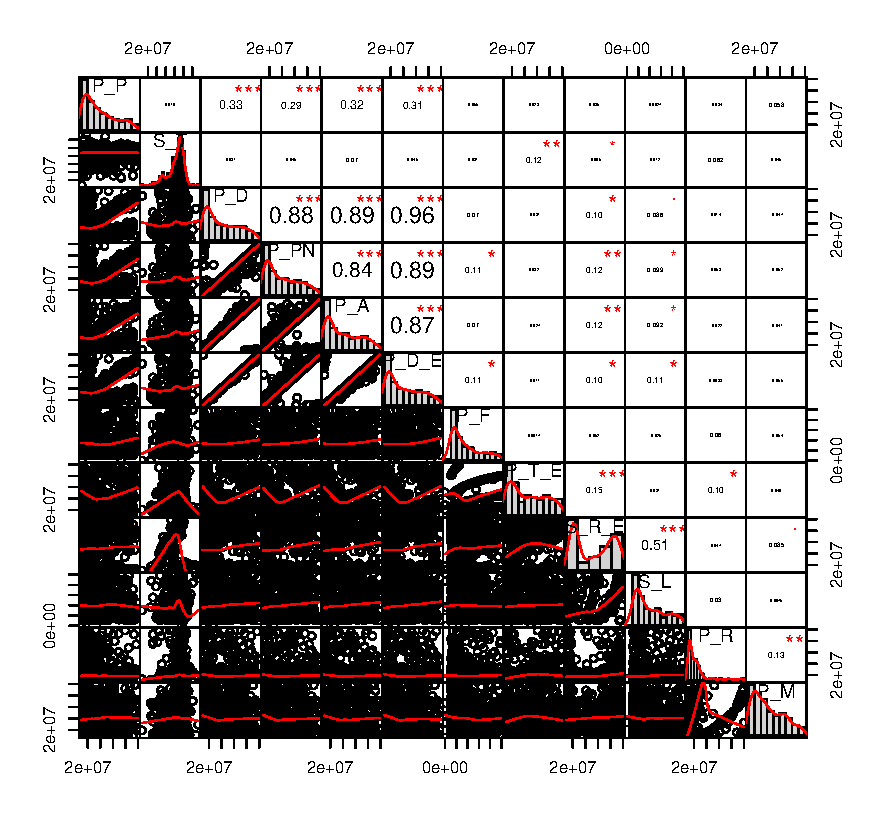
\includegraphics[width=1\textwidth]{Pic/Corr_chart.pdf}
\caption{The correlation chart for all the quantitative variables considered in this work}
\label{Corr_chart}
\end{center}
\end{figure}



\begin{figure}[h]
\begin{center}
\subfloat[]{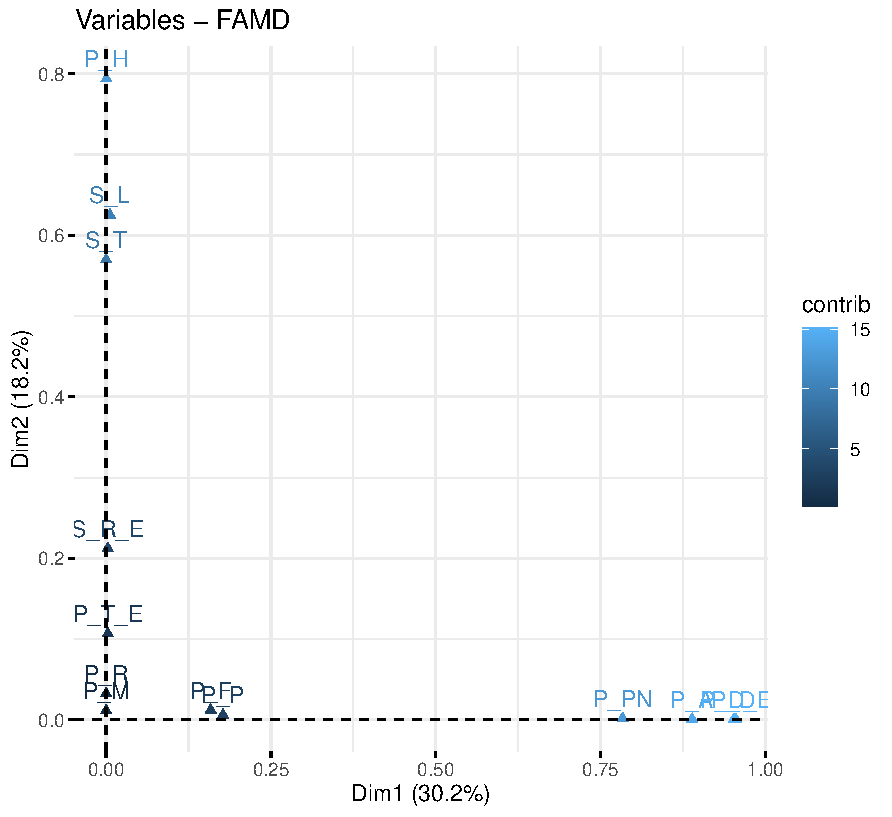
\includegraphics[width=0.5\textwidth]{Pic/FAMD_squared_loadings.pdf}}\\
\subfloat[]{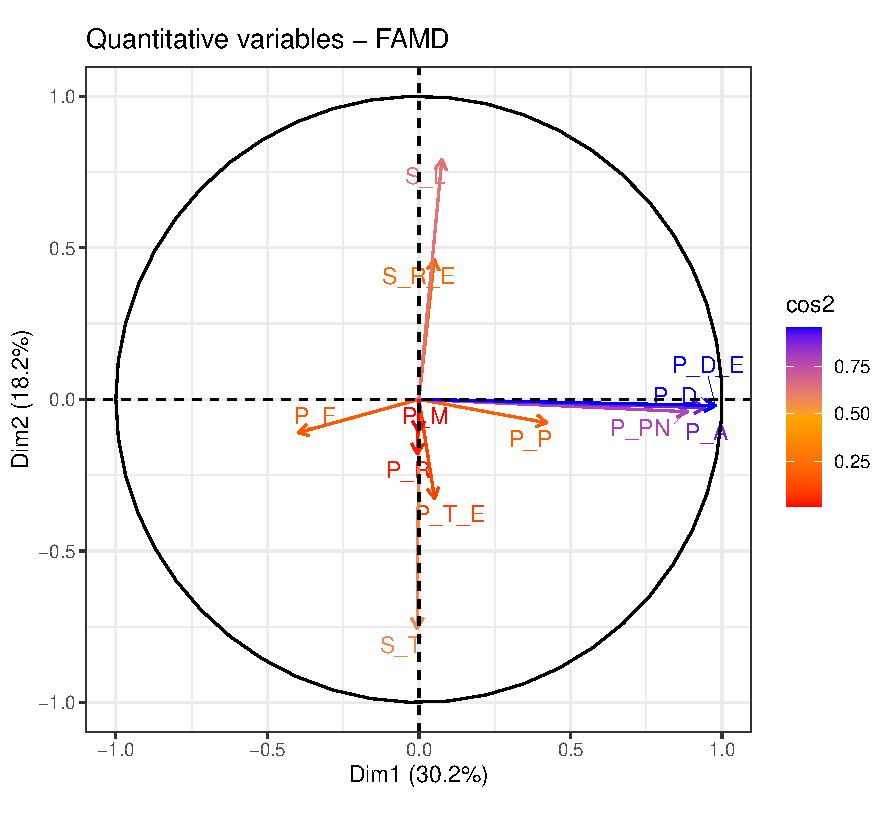
\includegraphics[width=0.5\textwidth]{Pic/FAMD_quantitative_variables.pdf}}
\subfloat[]{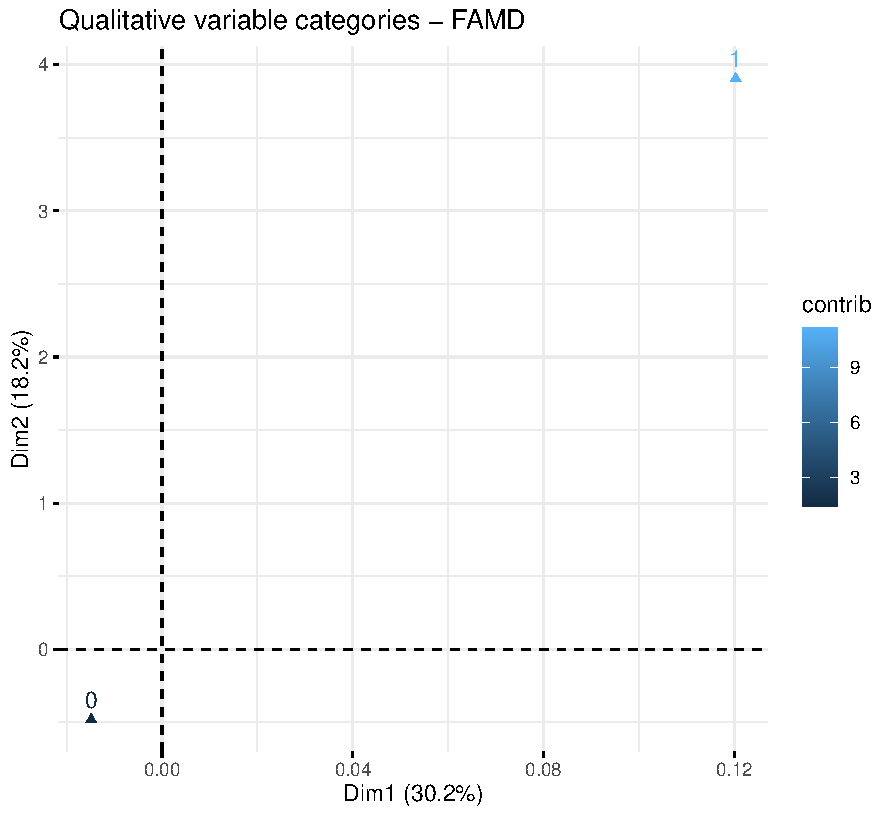
\includegraphics[width=0.5\textwidth]{Pic/FAMD_Qualitative_VAR.pdf}}\\
\caption{The FAMD analysis of the dataset: on the panel (a)  the relationship square, on  the panel (b) the correlation circle is provided and on panel (c) the representation of the categories is given.}
\label{PCA+SVM_PLOT}
\end{center}
\end{figure}

\clearpage

\subsection{Decision tree and random forest}
The first approach that was considered is the classification decision tree \footnote{In this work, for all the approaches undertaken, the training ensemble consist in a set of 350 exoplanets while the test one is composed by 150 items.}: as it can be seen from Fig \ref{DecisionTree}, where the decision tree is given accompanied by a plot that provides the variables importance,  the main discriminant parameters, as expected, are the planet temperature equilibrium $P\_T\_E$ and the stellar temperature $S\_T$: this features discriminates, as one expects, the largest part of the habitable planet from the non-habitable. The performance of this algorithm on this dataset, evaluated with a 10-fold cross-validation \footnote{For this procedure, applied to all algorithms here considered, the test set and the training sets where reshuffled 10 times by modifying the numerical seed by which the exoplanets are assigned to the training or to the test set. The model was than trained again with the reshuffled set. The confusion matrices reported here are the sum of the 10 forecast on the test set obtained.}, is reported in Fig \ref{Decision_tree_performances} and in the table \ref{perf_table}. Next, in order to improve the performance of this classification, the random forest was considered. As shown in Fig. \ref{Random_forest_tree_perfs} the main parameters for this algorithm were previously checked. Its results are reported in Fig \ref{Random_forest_tree_results}: here the most important variable is still $P\_T\_E$ followed by the $S\_T$.  Moreover  as one can note from Fig \ref{Random_forest_tree_results} the performances are slightly improved with respect to the ones reported in Fig \ref{Decision_tree_performances}.  Such improvement is captured by the accuracy and $\phi$ factors reported in table \ref{perf_table}. Finally it is worth noting that, although  different features were also considered and the output of the response function has a larger set,  a similar hierarchy  among the variable importance for the random forest algorithm was obtained by Saha et al. \cite{saha2018machine}: in their paper the highest variable importance, via random forest algorithm,  is assigned to the mean planet temperature at surface followed by the stellar magnitude with respect to the planet (between these two there are other features strictly connected to the planet surface temperature). The last quantity is strictly connected to the stellar temperature and to the stellar spectral type. Moreover also in their study the mean distance between the planet and host star plays a minor role.


\begin{figure}[h]
 \centering
\begin{center}
\subfloat[]{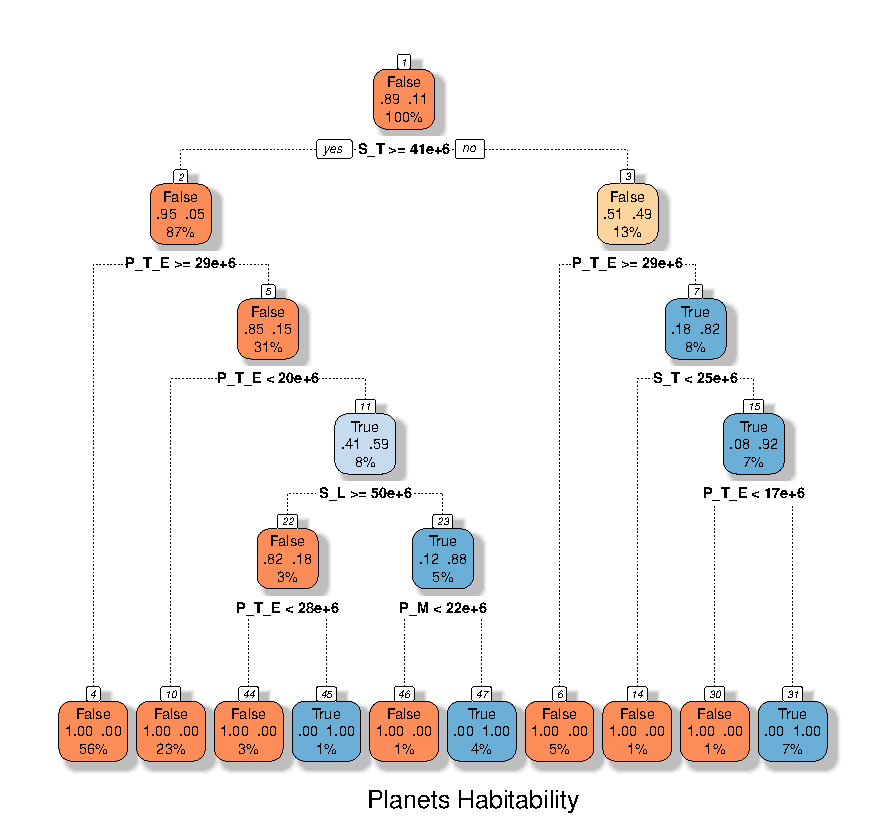
\includegraphics[width=0.5\textwidth]{Pic/DecisionTree.pdf}}
\subfloat[]{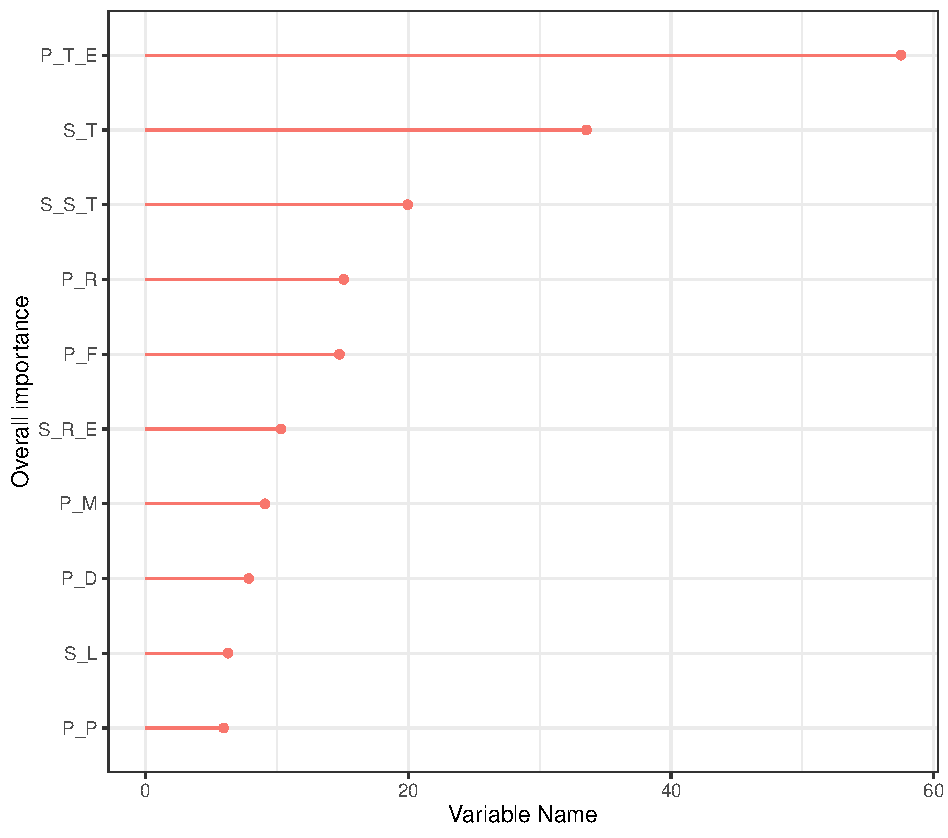
\includegraphics[width=0.5\textwidth]{Pic/Var_imp_dec_tree.pdf}}
\caption{The classification of exoplanets habitability obtained by the decision tree algorithm (\textit{True} stands for habitable while \textit{False} not habitable). The units of measure are reported in the table \ref{features_table}. In the  left panel (a) the decision tree representation is plotted: the highest number in each box refers to the output of the classifier give the condition reported on his bottom, the two number in the middle the percentages of the splitting and the last number the overall percentage of the planes classified by the node. Note that, since only boxes for which more than 5 items were considered, the overall sum is lower than $100 \%$. In the lower panel (b) is reported the overall importance of each variable.}
\label{DecisionTree}
\end{center}
\end{figure}


\begin{figure}[htp]
  \centering
\subfloat[]{\label{Decision_Tree_FINAL_CV}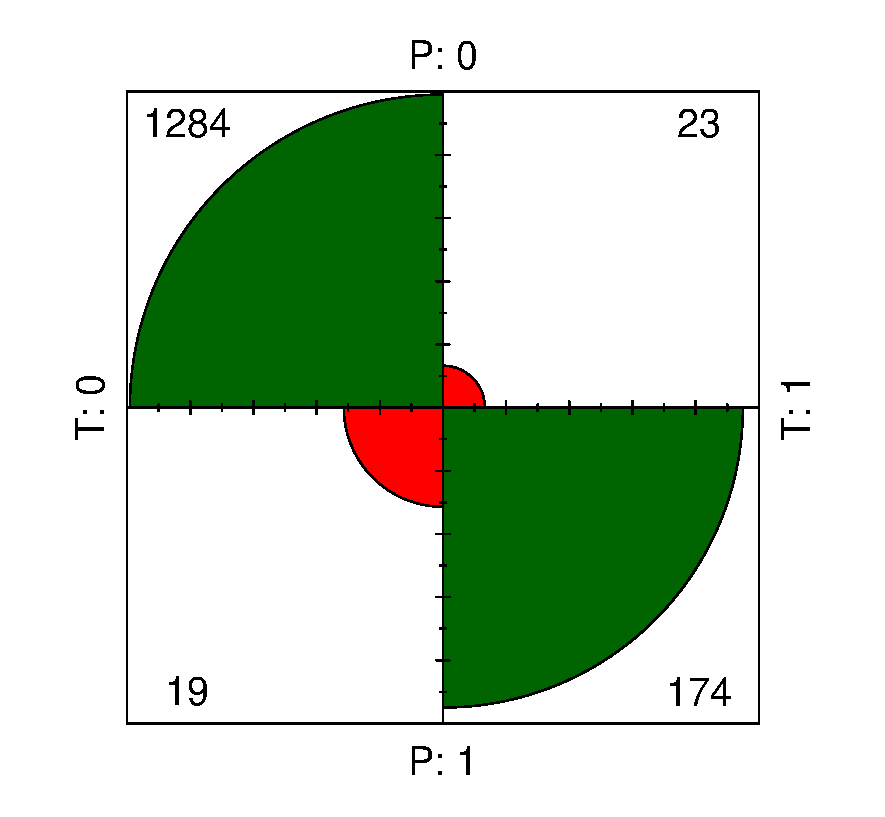
\includegraphics[width=0.6\textwidth]{Pic/Decision_Tree_FINAL_CV.pdf}}\\
\subfloat[]{\label{Decision_Tree_FINAL_CV}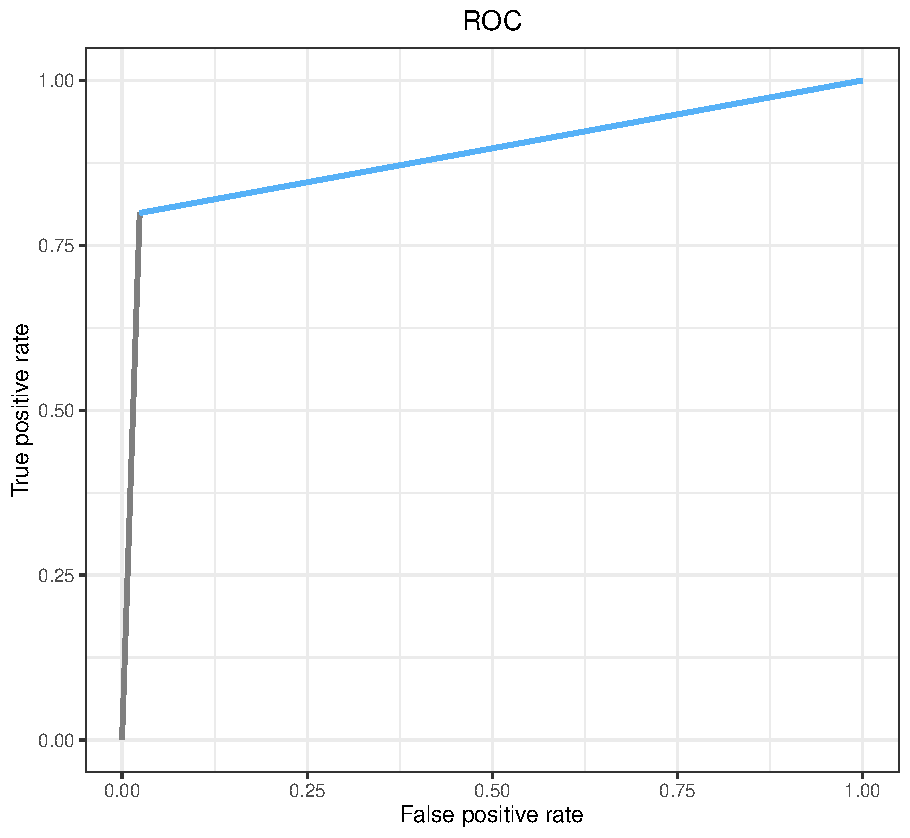
\includegraphics[width=0.6\textwidth]{Pic/Decision_Tree_FINAL_ROC.pdf}}
\caption{The performances of the decision tree algorithm on the habitability of exoplanets as given by the confusion matrix (upper panel) and ROC curve (lower panel) as obtained by a 10-fold cross validation. A predicted (P) habitable exoplanet is classified as True (T) while a test (T) non-habitable exoplanet is classified as False (F) }
\label{Decision_tree_performances}
\end{figure}

\begin{figure}[h]
  \centering
\subfloat[]{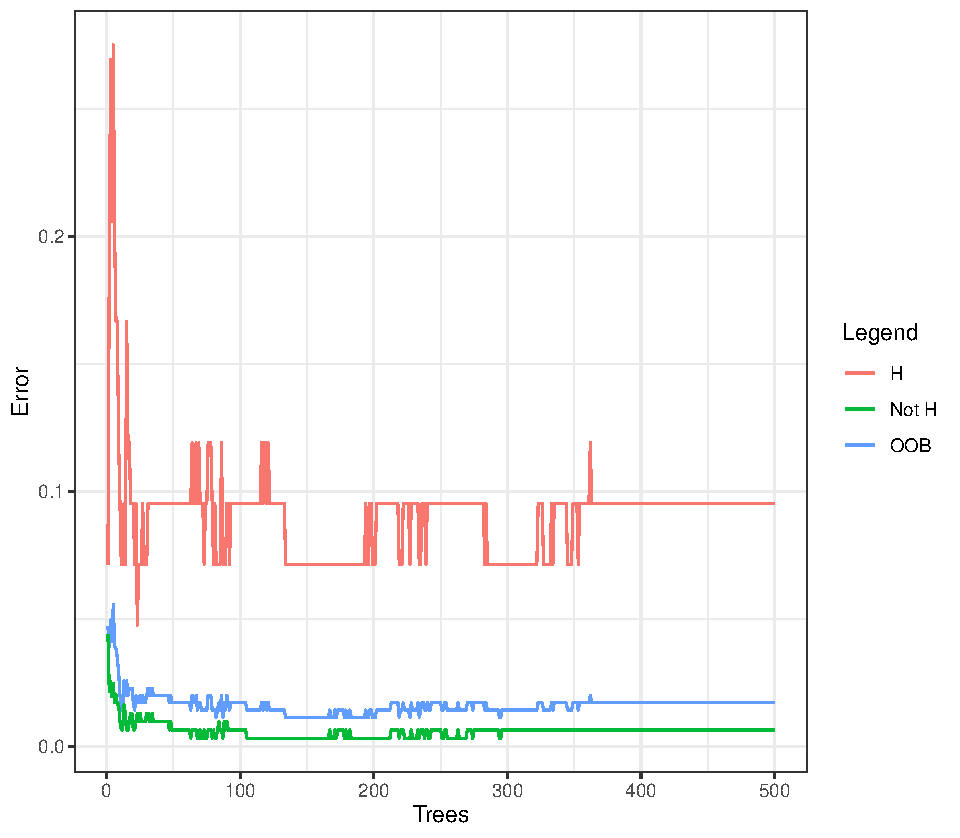
\includegraphics[width=0.5\textwidth]{Pic/Random_forest_trees.pdf}}
\subfloat[]{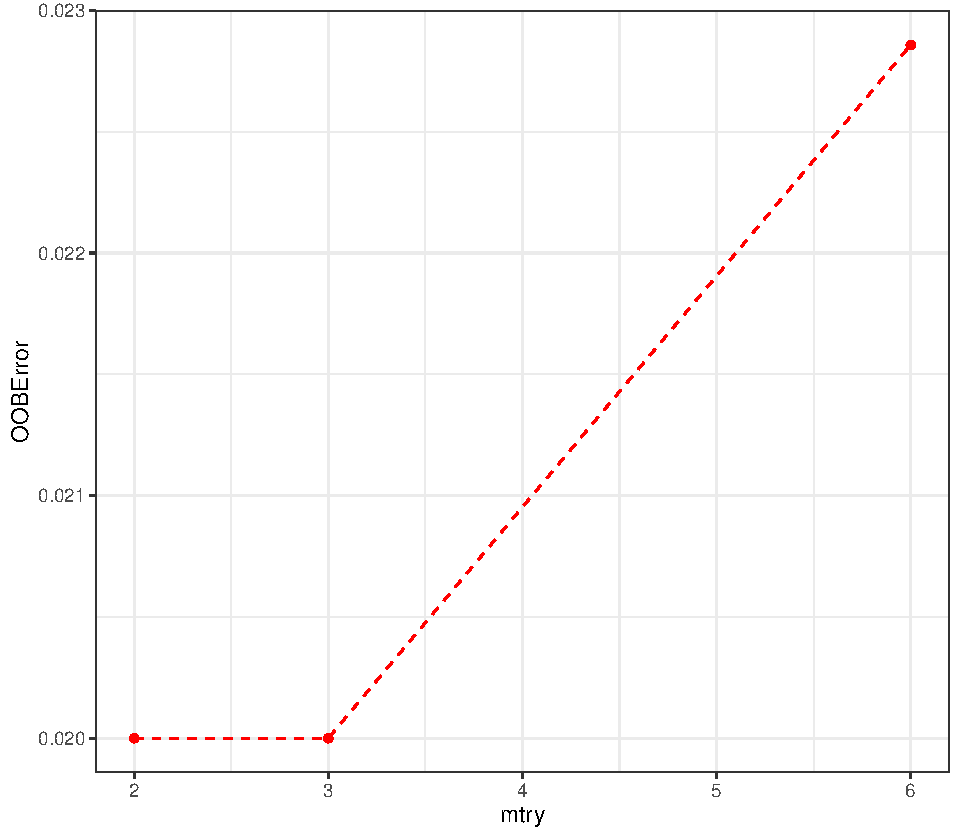
\includegraphics[width=0.5\textwidth]{Pic/mtry_Random_forest.pdf}}
\caption{The performances of the random forest algorithm as the main parameters are modified: as the ensemble grew (panel a) accompanied by the optimization of the number of variables available (mtry). For the calculations presented in this work an ensemble of 500 trees (the default one) was considered while the mytry parameter was set equal to 4.}
\label{Random_forest_tree_perfs}
\end{figure}

\begin{figure}[h]
  \centering
\subfloat[]{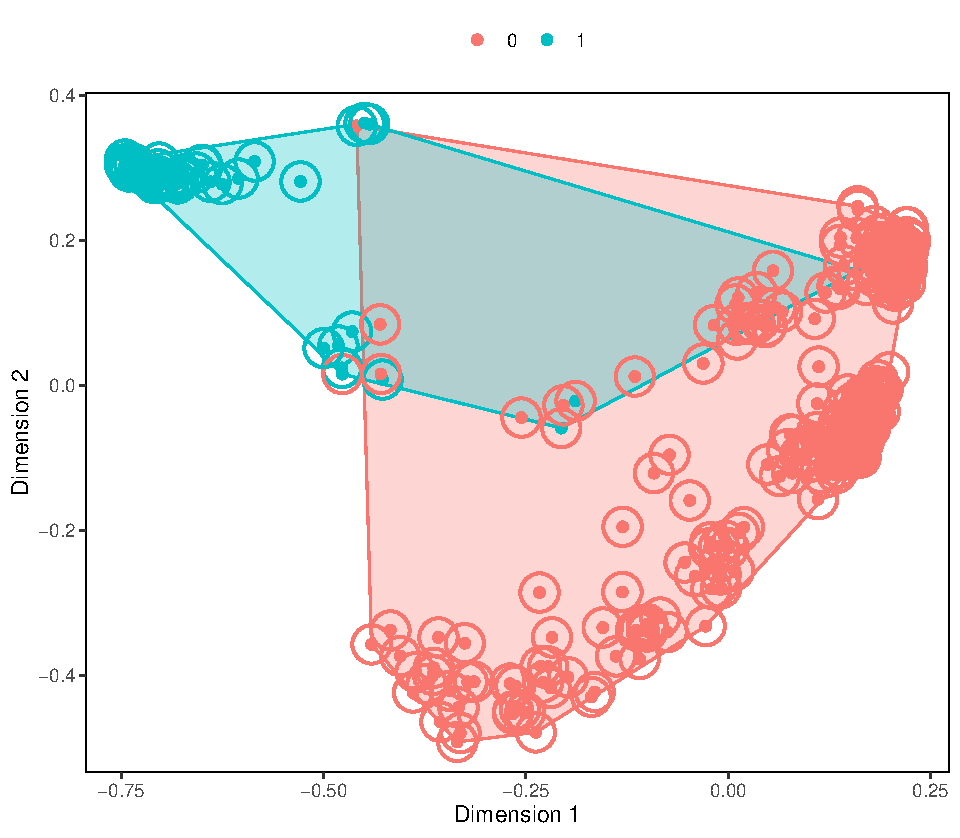
\includegraphics[width=0.8\textwidth]{Pic/Proximity_Random_forest.pdf}}\\
\subfloat[]{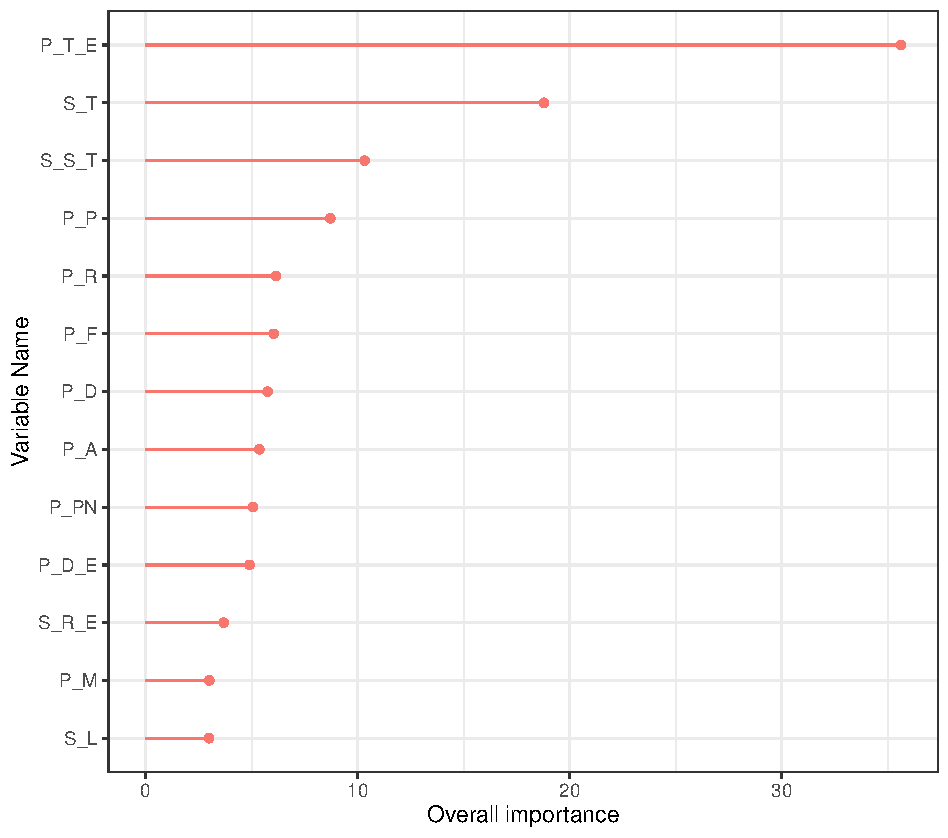
\includegraphics[width=0.8\textwidth]{Pic/Random_forest_importance.pdf}}
\caption{Main results achieved with the random forest algorithm: on the upper panel (a) the random Forest proximity scores is reported while on the bottom panel (b) the overall importance of each variable is plotted. Note that in this case the hierarchy importance of the variables is slightly changed with respect to the Fig \ref{DecisionTree} }
\label{Random_forest_tree_results}
\end{figure}

\begin{figure}[h]
  \centering
\subfloat[]{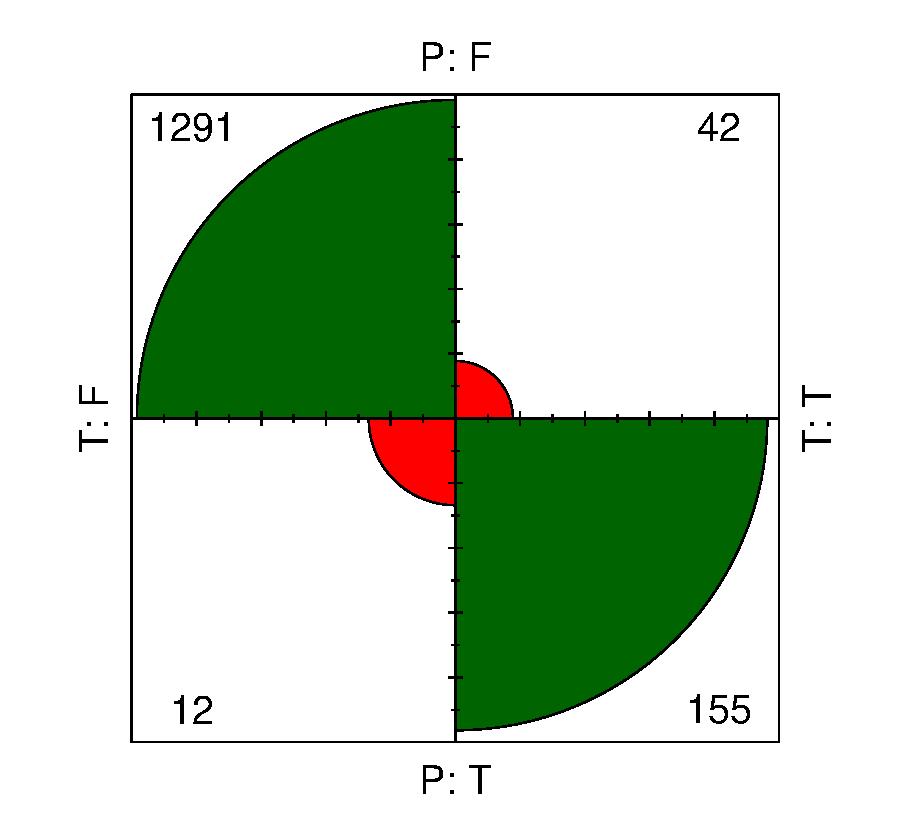
\includegraphics[width=0.6\textwidth]{Pic/Random_Forest_FINAL_CV.pdf}}\\
\subfloat[]{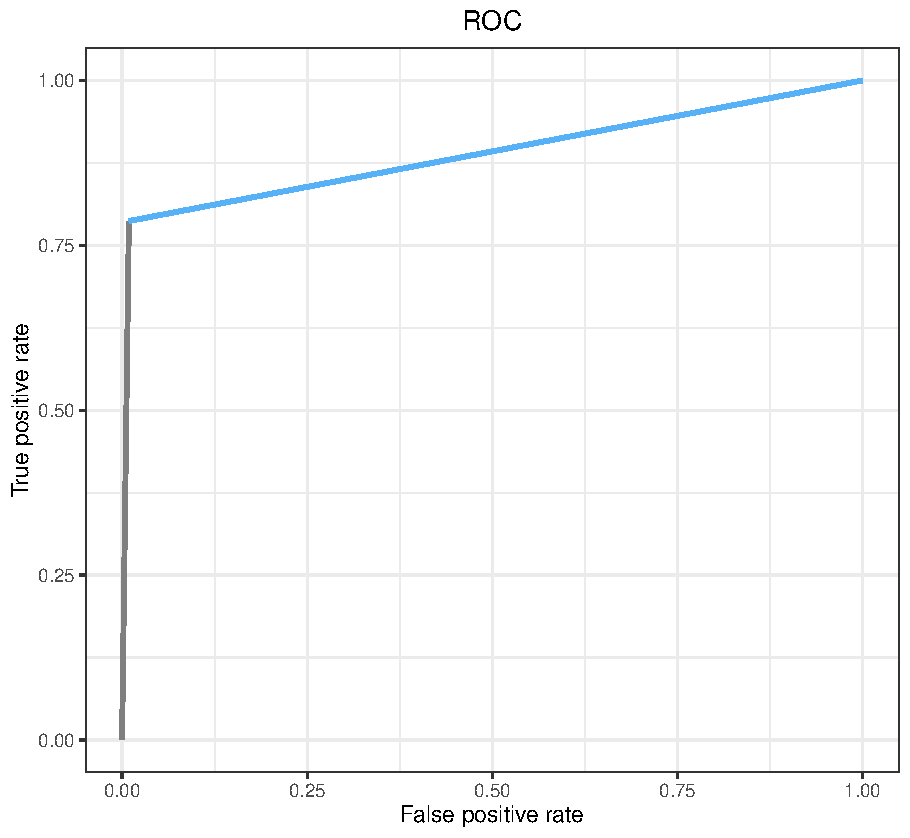
\includegraphics[width=0.6\textwidth]{Pic/Random_Forest_FINAL_ROC.pdf}}
\caption{The performances of the random forest algorithm on the habitability of exoplanets as given by the confusion matrix (upper panel) and ROC curve (lower panel) as obtained by a 10-fold cross validation. A predicted (P) habitable exoplanet is classified as True (T) while a test (T) non-habitable exoplanet is classified as False (F)}
\label{Random_forest_tree_results}
\end{figure} 

\clearpage 


\subsection{Support Vector Classifiers}
Next the SVM classification algorithm was considered: the most important parameters , in this case the budget and the polynomial degree , were tuned (see Fig. \ref{SVM_tuning}). The performances of this approach are reported in the Fig. \ref{SVM_results} and in the Tab. \ref{perf_table}: these seems to be worst with respect to the decision tree and random forest. In order to survey the origin of this bad performance the dimensionality reduction with principal component analysis (PCA) was performed in order to obtain a 2D plot of the decision boundary \footnote{Since the planet habitability is a categorical variable a particular library was used: indeed the PCAmixdata package provides the function \textit{PCAmix()} that manage the quantitative variables with the principal component analysis (PCA), while the qualitative variables are undertaken via the multiple correspondence analysis (MCA)}. As can be seen from Fig. \ref{PCA+SVM_PLOT} \footnote{The degree and the budget for the SVM used here  were tuned also in this case: the optimized parameters were 2 for the polynomial and 4 for the budget} the habitable and non-habitable exoplanets sets, also if the dimensions are reduced, are largely overlapping and the decision boundary is complex: this reduce the performance of the algorithm. This behaviour of SVM was also pointed out by Saha et al. \cite{saha2018machine}. However as showed in Fig \ref{SVM+PCA_results} and in the Tab. \ref{perf_table} the performance of the SVM classification are improved when the PCA is previously undertaken \footnote{In principle, on the basis of the variable importance previously obtained with the random forest, one can consider to reduce the dimensionality of the set by taking only the $P\_T\_E$ and the $S\_T$ features: in this case a better performance of SVM is expected}


\begin{figure}[h]
\begin{center}
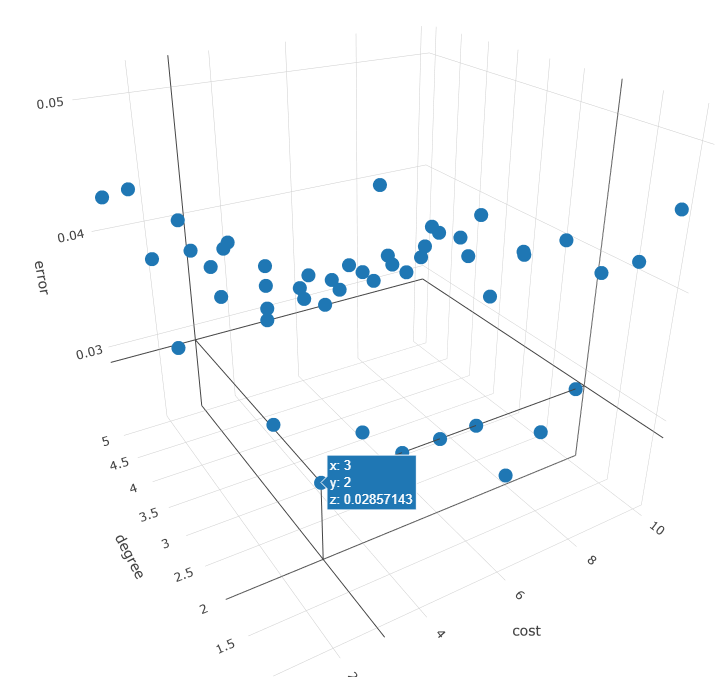
\includegraphics[width=0.8\textwidth]{Pic/SVM_tuning.png}
\caption{The tuning of the budget parameter and the polynomial degree for the SVM classification algorithm. The selected point (x represents the budged while y the polynomial degree) is the parameter set chosen for this work}
\label{SVM_tuning}
\end{center}
\end{figure}

\begin{figure}[h]
  \centering
\subfloat[]{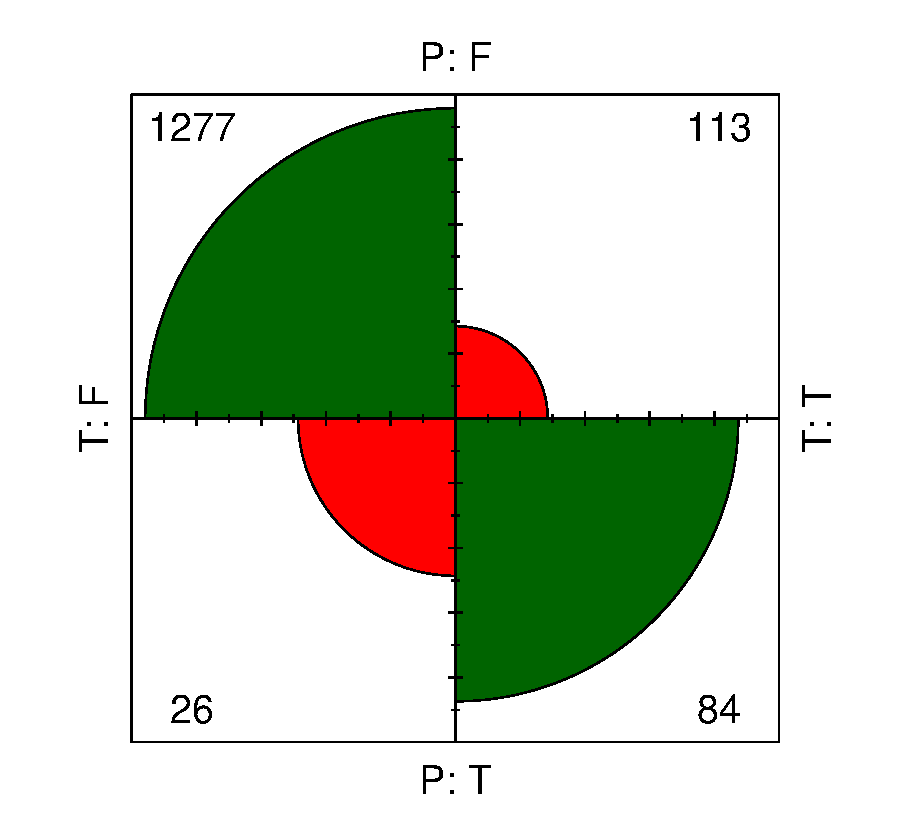
\includegraphics[width=0.6\textwidth]{Pic/SVM_FINAL_CV.pdf}}\\
\subfloat[]{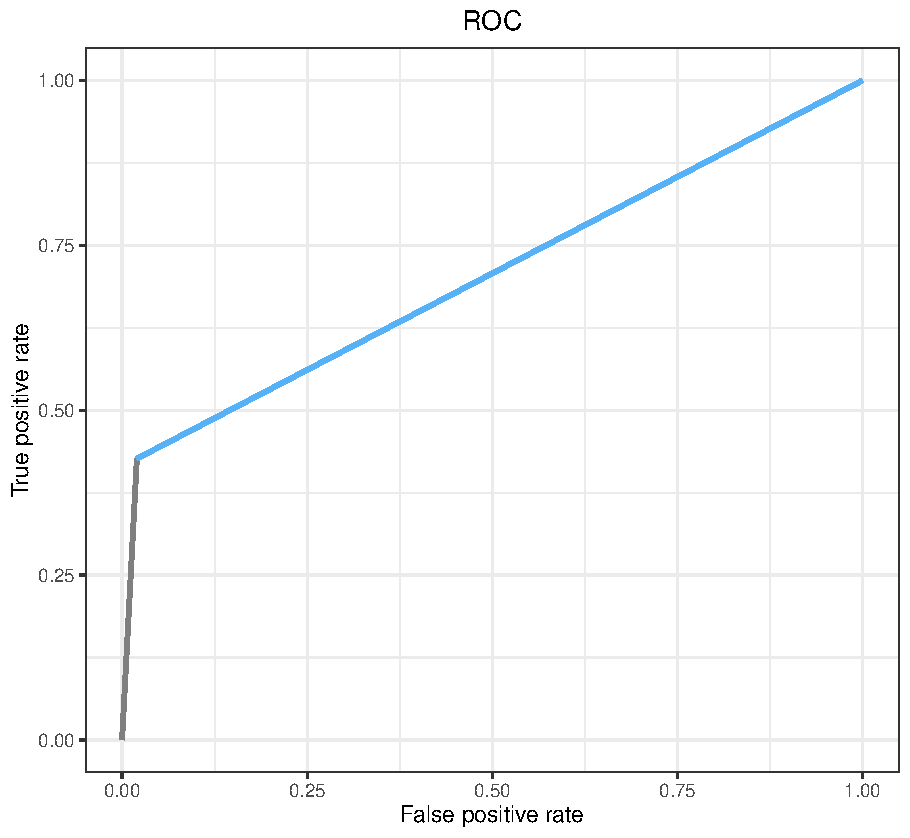
\includegraphics[width=0.6\textwidth]{Pic/SVM_FINAL_ROC.pdf}}
\caption{The performances of the SVM on the habitability of exoplanets as given by the confusion matrix (upper panel) and ROC curve (lower panel) as obtained by a 10-fold cross validation.  A predicted (P) habitable exoplanet is classified as True (T) while a test (T) non-habitable exoplanet is classified as False (F).}
\label{SVM_results}
\end{figure}

\begin{figure}[h]
\begin{center}
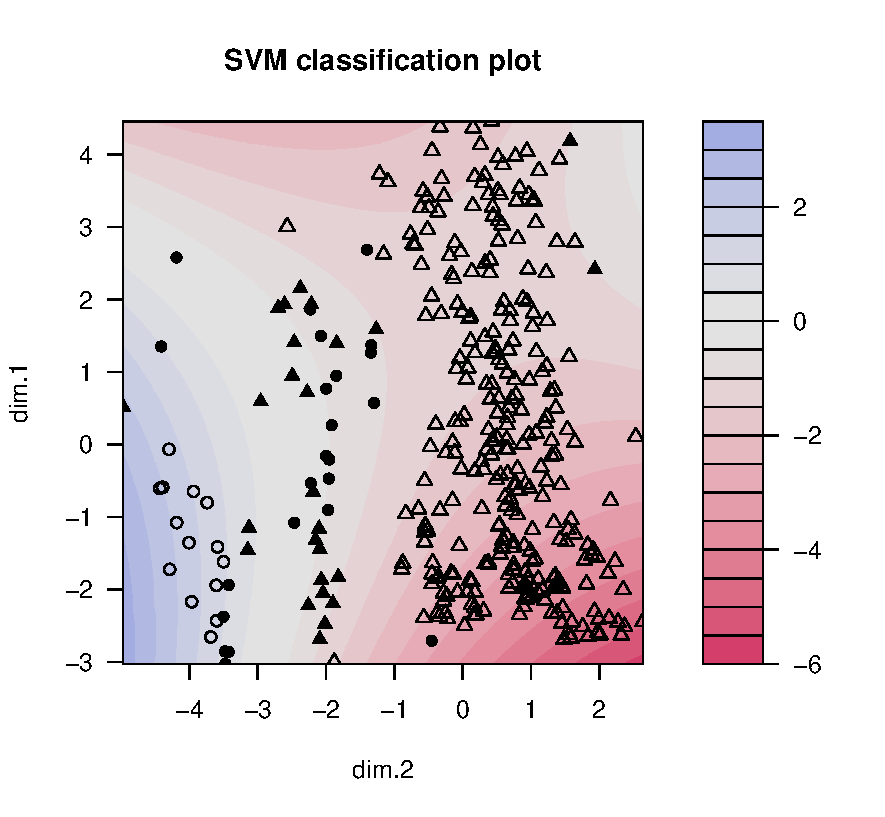
\includegraphics[width=1\textwidth]{Pic/PCA+SVM_PLOT.pdf}
\caption{The SVM classification applied to the training set after the dimensionality reduction via PCA. The filled symbols (triangle for not habitable and circle for habitable) represent the support vectors }
\label{PCA+SVM_PLOT}
\end{center}
\end{figure}



\begin{figure}[h]
  \centering
\subfloat[]{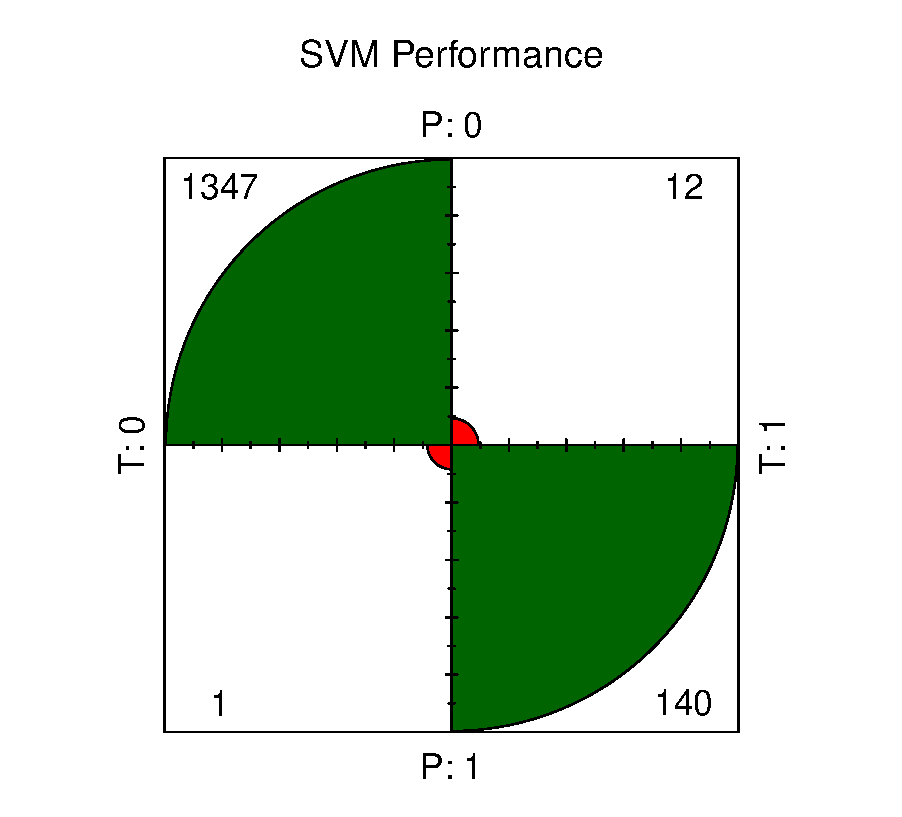
\includegraphics[width=0.6\textwidth]{Pic/SVM_PCA_CV.pdf}}\\
\subfloat[]{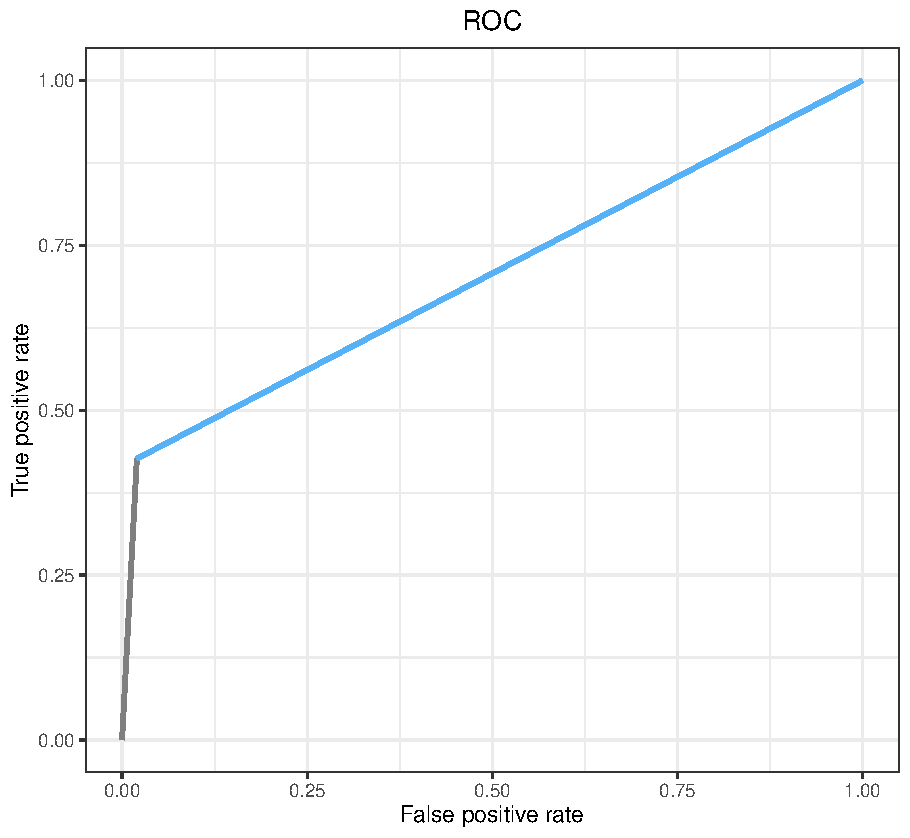
\includegraphics[width=0.6\textwidth]{Pic/SVM_PCA_ROC.pdf}}
\caption{The performances of the SVM on the habitability of exoplanets (as obtained by a 10-fold cross validation) once the the dimensionality reduction via was applied (to 2 dimension): on the panel (a) the confusion matrix is given  while on panel (b) the ROC curve (lower panel) is reported. A predicted (P) habitable exoplanet is classified as True (T) while a test (T) non-habitable exoplanet is classified as False (F)}
\label{SVM+PCA_results}
\end{figure}

\clearpage


\subsection{Logistic regression}
Beside the approaches previously described, the logistic classification was also undertaken: its performances are reported in Fig. \ref{logistic_performances} and in the Tab. \ref{perf_table}: the overall result seems better with respect to the SVM algorithm but definitely lower with respect to the decision tree and the random forest algorithms. 

\begin{figure}[h]
  \centering
\subfloat[]{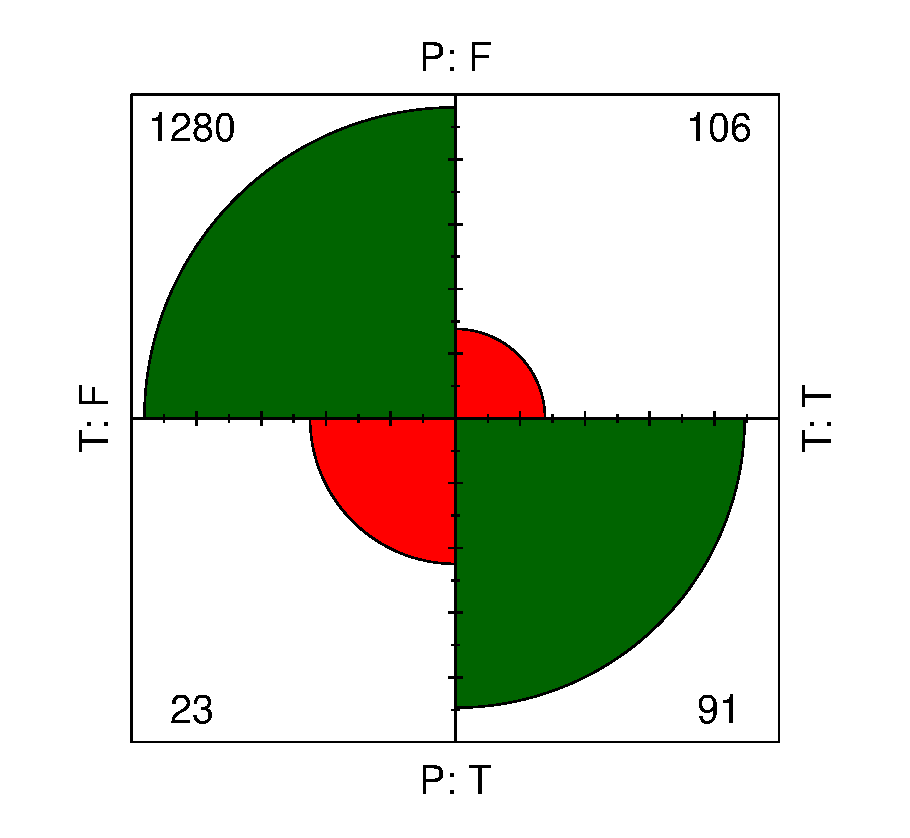
\includegraphics[width=0.6\textwidth]{Pic/LOG_FULL.pdf}}\\
\subfloat[]{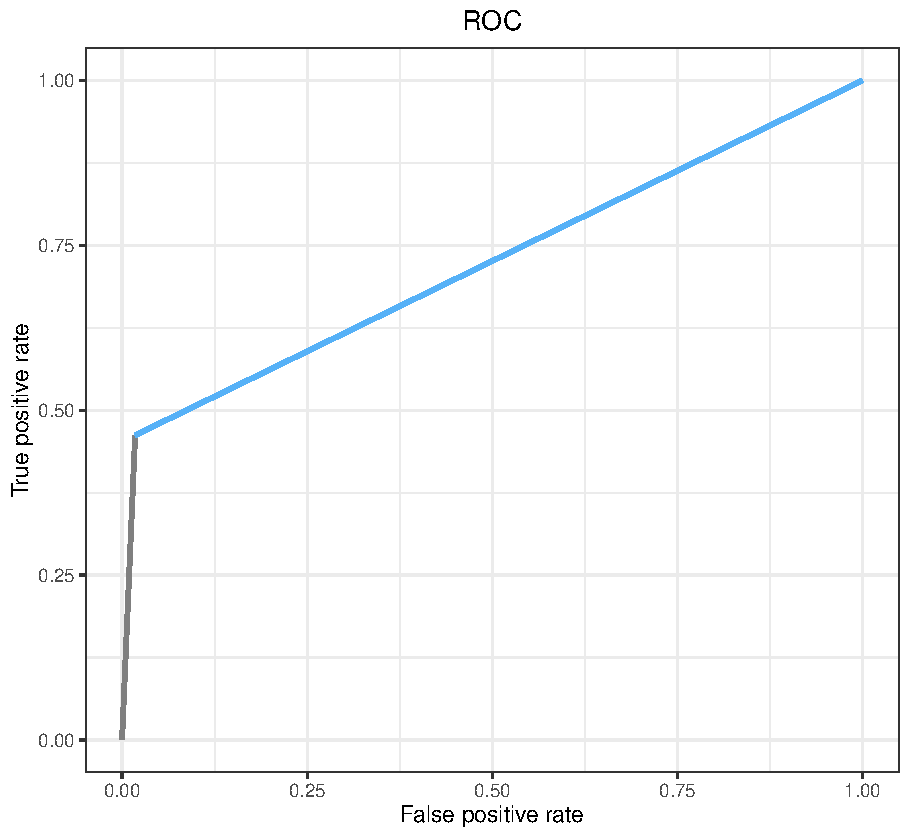
\includegraphics[width=0.6\textwidth]{Pic/LOG_FULL_ROC.pdf}}
\caption{The performances of the multiple logistic regression on the habitability of exoplanets (as obtained by a 10-fold cross validation) once the the dimensionality reduction via was applied (to 2 dimension): on the panel (a) the confusion matrix is given  while on panel (b) the ROC curve (lower panel) is reported.  A predicted (P) habitable exoplanet is classified as True (T) while a test (T) non-habitable exoplanet is classified as False (F)}
\label{logistic_performances}
\end{figure}

\clearpage



\subsection{Linear and quadratic analysis}
Finally the liner and quadratic discriminant analysis algorithms were used: their performances are plotted in Fig. and reported in Fig. \ref{LDA+QDA_results}. As it possible to see from the Tab. \ref{perf_table} and \ref{LDA+QDA_results} the performances of the quadratic discriminant analysis are better, but not enought to pair the random forest or the decision tree. The fact that the QDA algortim performs better with respect to LDA is consistent with the previous finding obtained for the SVM where the tuned polynomial for the decision boundary was of degree two \footnote{The analogy between these two methods basically ends here since they are two very different approaches for the estimation of the decision boundary}. A deeper inspection of the hyperspace confirmed this conjecture: in Fig. \ref{QDA_project_FULL} the different projections are given while in Fig. \ref{QDA_project_red} the one in which the $P\_T\_E$ and the $S\_T$ are considered, is given. It is worth noting that the latter is the one with the lowest error, in accordance with the variable importance hierarchy obtained with the random forest.  

\begin{figure}[h]
  \centering
\subfloat[]{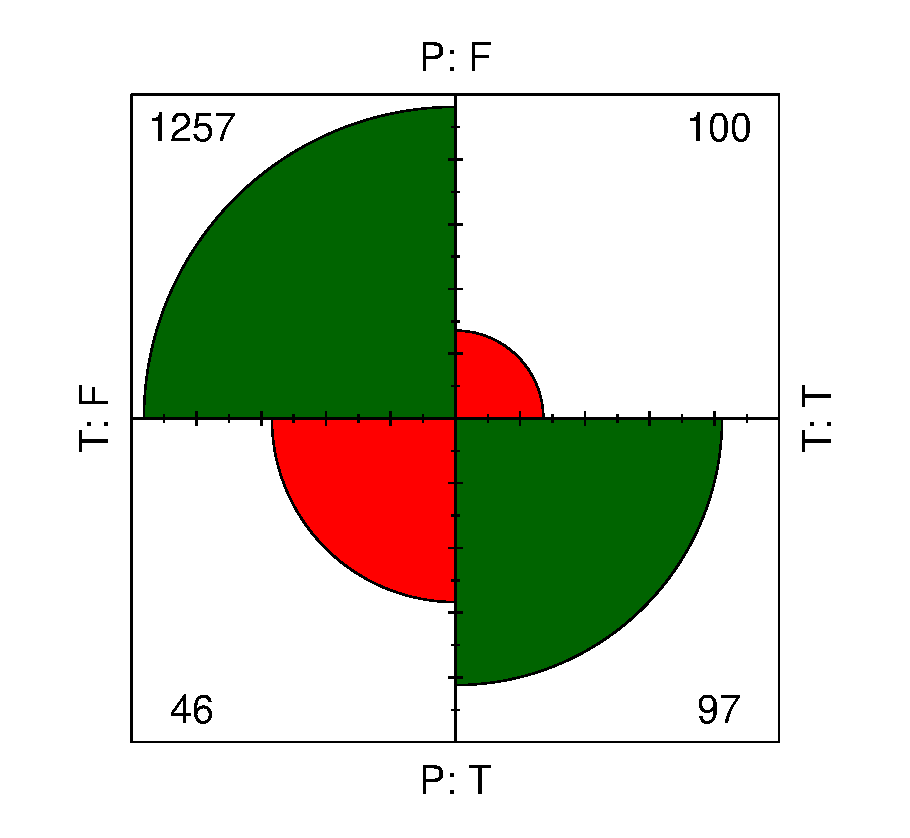
\includegraphics[width=0.4\textwidth]{Pic/LDA_FULL_CV.pdf}}
\subfloat[]{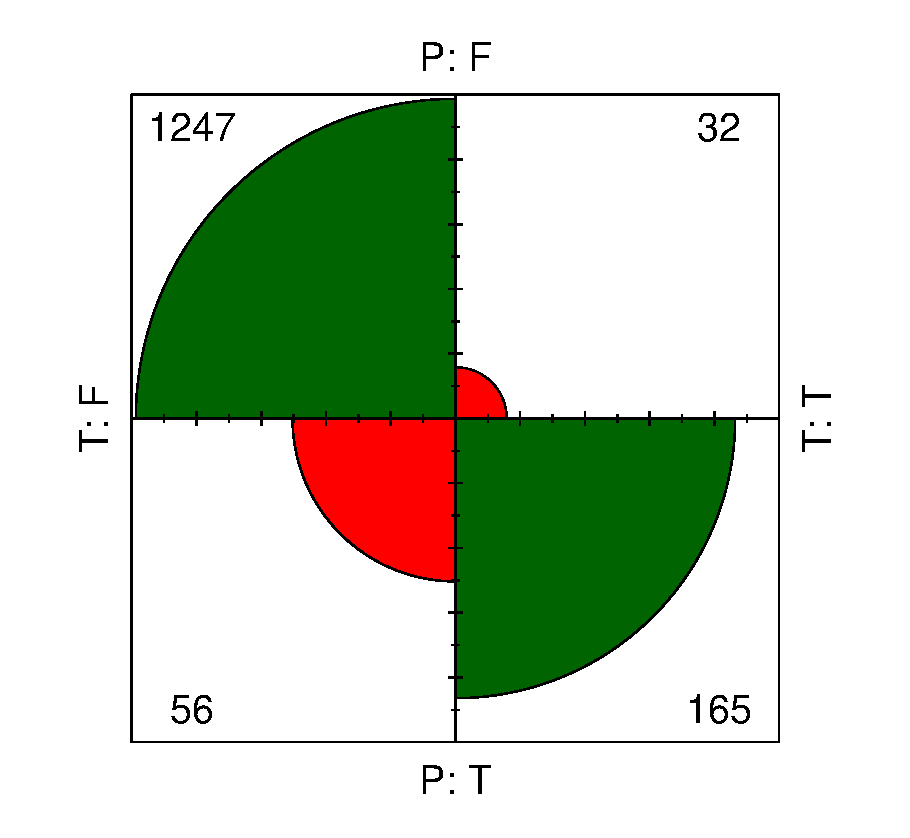
\includegraphics[width=0.4\textwidth]{Pic/QDA_FULL_CV.pdf}}\\
\subfloat[]{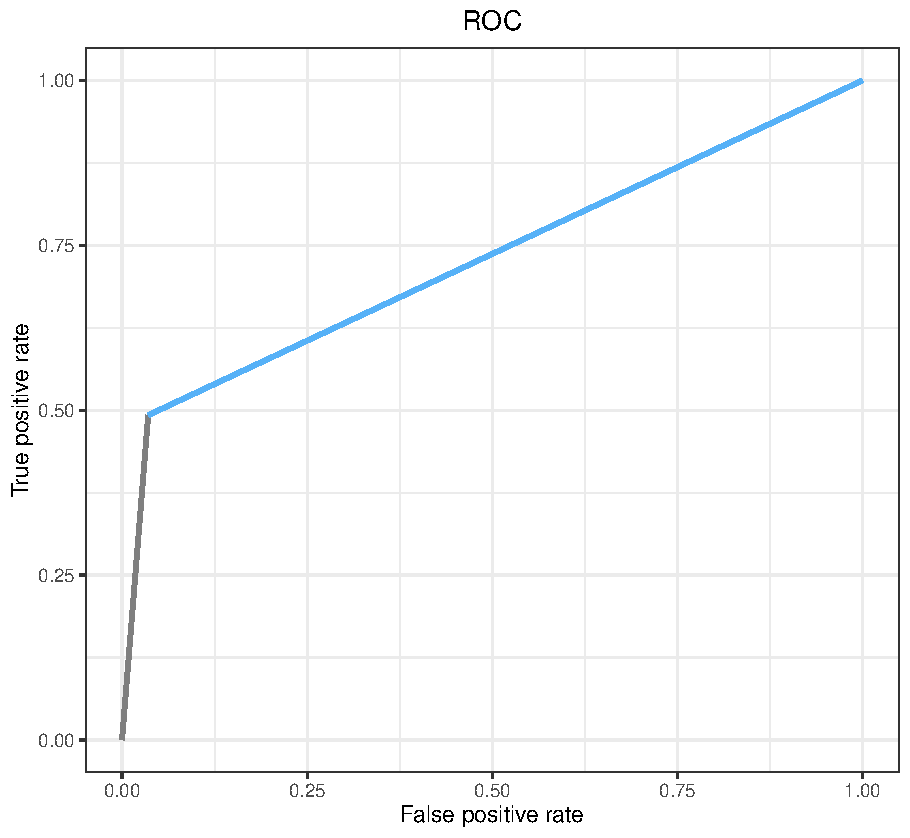
\includegraphics[width=0.4\textwidth]{Pic/LDA_FULL_ROC.pdf}}
\subfloat[]{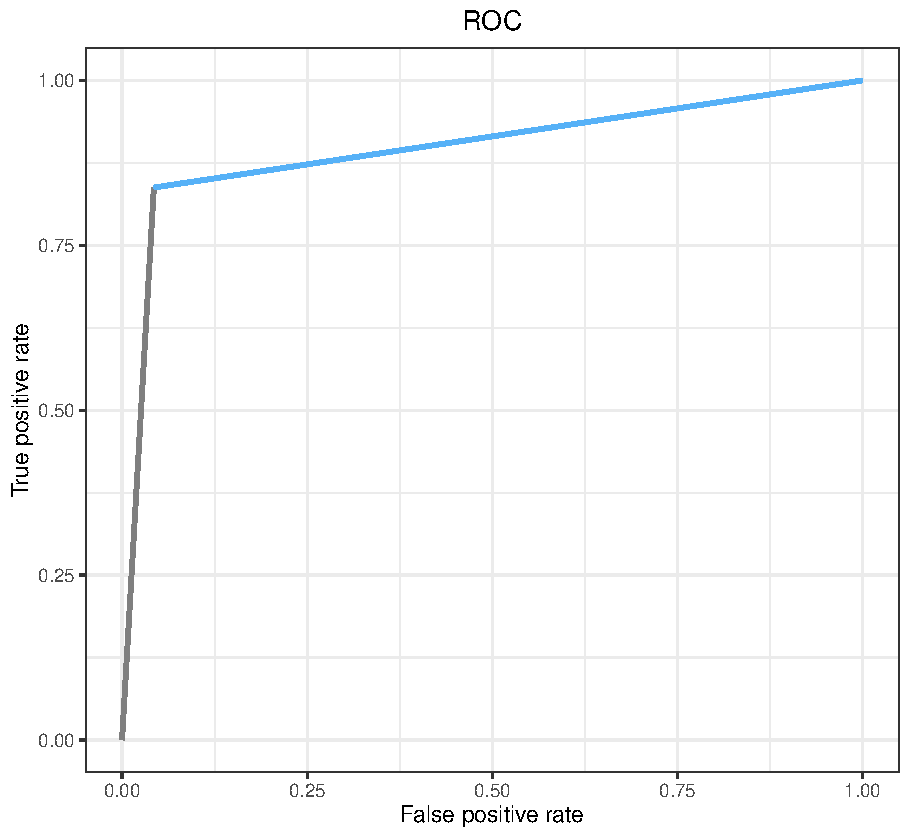
\includegraphics[width=0.4\textwidth]{Pic/QDA_FULL_ROC.pdf}}
\caption{The performances of the LDA (left panels a and c) and QDA (right panels b and d) on the habitability of exoplanets as obtained by a 10-fold cross validation.   A predicted (P) habitable exoplanet is classified as True (T) while a test (T) non-habitable exoplanet is classified as False (F)}
\label{LDA+QDA_results}
\end{figure}



\begin{figure}[h]
\begin{center}
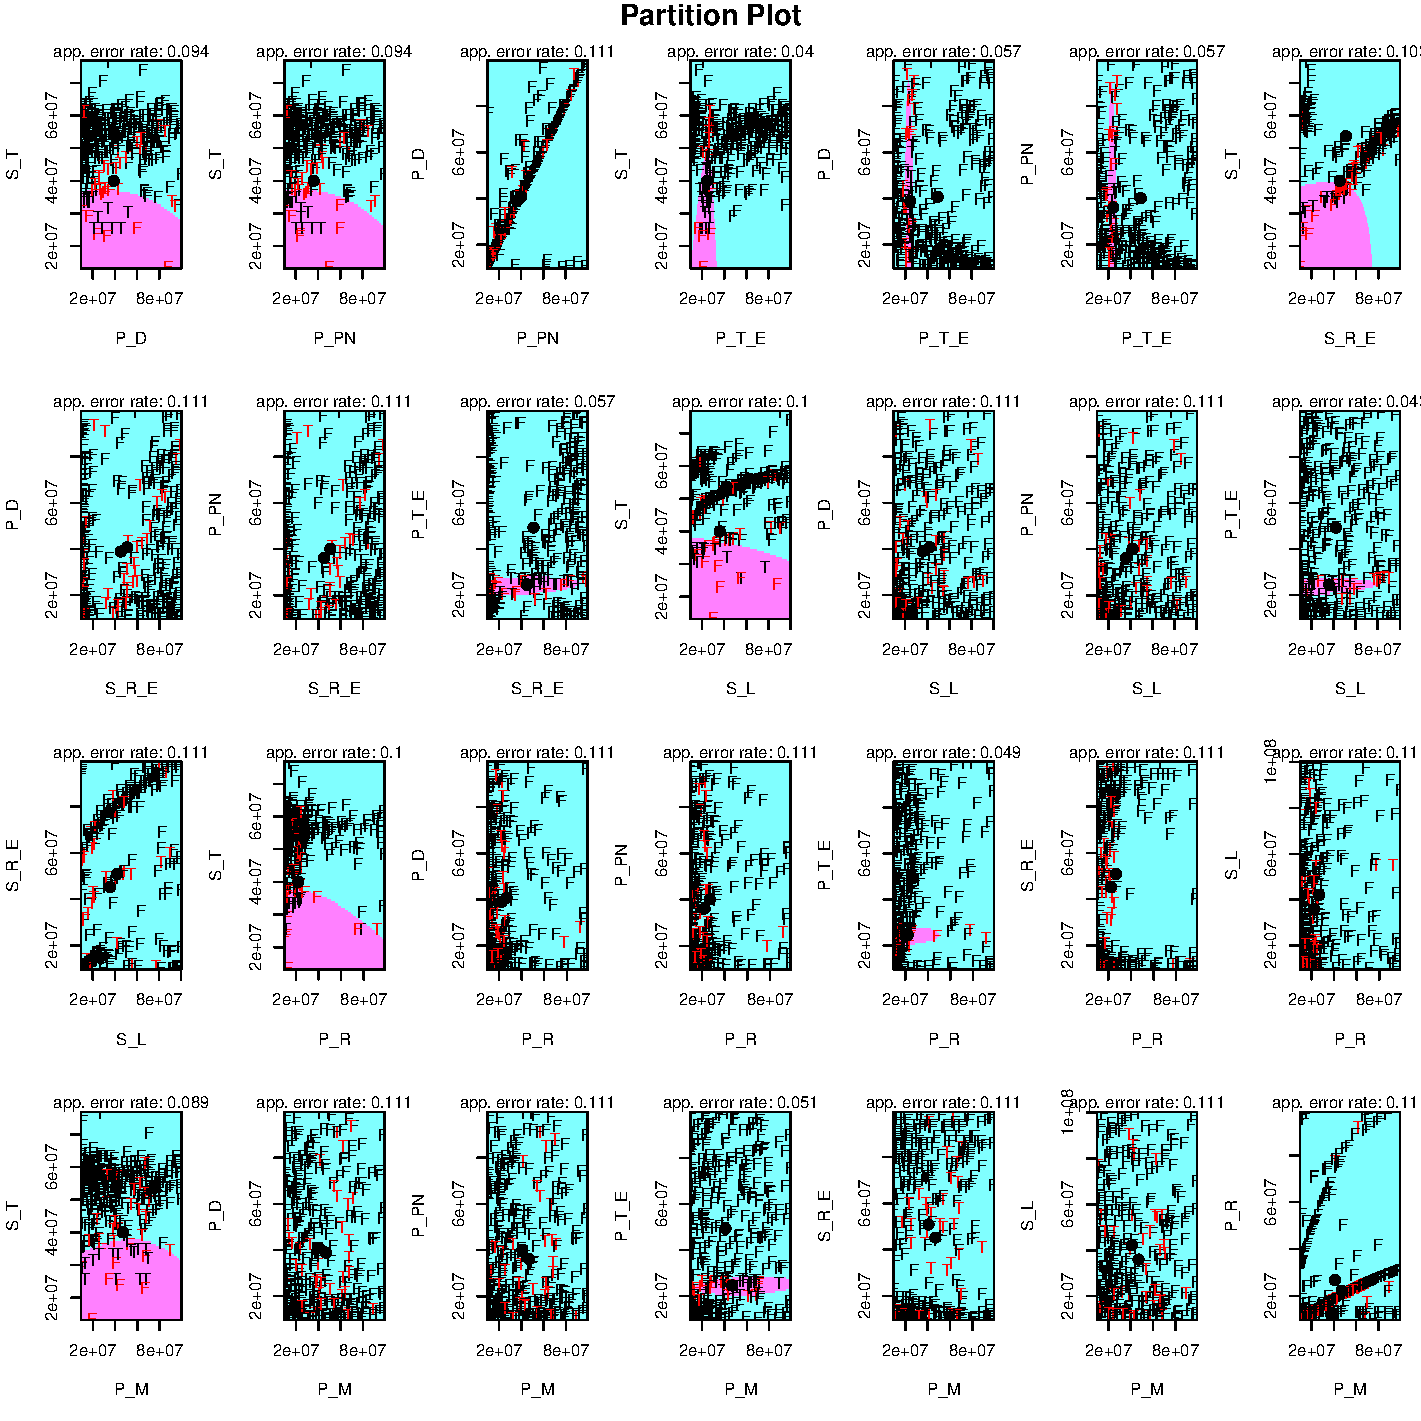
\includegraphics[width=1\textwidth]{Pic/QDA_project_FULL.pdf}
\caption{The projection on different couple of axes for the QDA classification. A predicted (P) habitable exoplanet is classified as T while a test (T) non-habitable exoplanet is classified as F. The red labels refer to the misclassified exoplanets}
\label{QDA_project_FULL}
\end{center}
\end{figure}

\begin{figure}[h]
\begin{center}
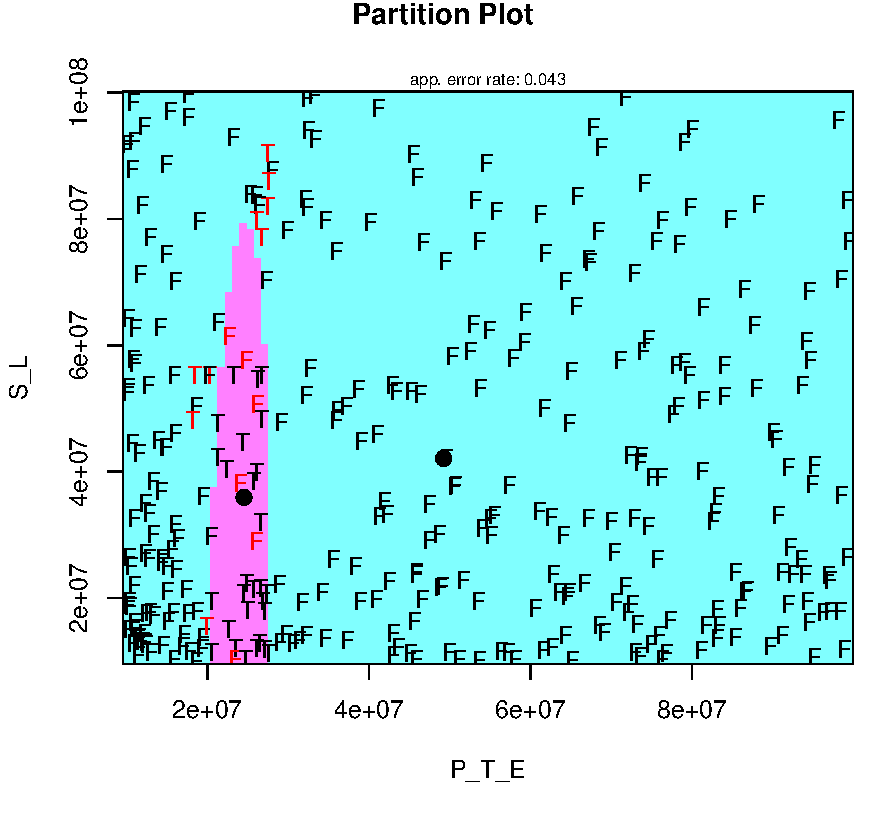
\includegraphics[width=1\textwidth]{Pic/QDA_project_RED.pdf}
\caption{The projection of QDA classification on the $P\_T\_E$ and $S\_L$ axes. Note, as showed in Fig. \ref{QDA_project_FULL} that this is the projection with the lowest error (consistently with the results of random forest algorithm). A predicted (P) habitable exoplanet is classified as True (T) while a test (T) non-habitable exoplanet is classified as False (F)}
\label{QDA_project_red}
\end{center}
\end{figure}


\clearpage

\begin{table}[]
\caption{The performances of the algorithm here considered as evaluated by their accuracy (compared to the no-information rate NIR) and the $\phi$ factor} 
\begin{center}
\begin{tabular}{c||c|c|c}
{\color[HTML]{CB0000} \textbf{Algortim}} & {\color[HTML]{CB0000} \textbf{Accuracy}} & {\color[HTML]{CB0000} \textbf{NIR}} & {\color[HTML]{CB0000} \textbf{$\phi$}} \\ \hline\hline
Decision tree                            & 0.952                                    & 0.867                               & 0.790                                  \\ \hline
Random forest                            & 0.964                                    & 0.869                               & 0.835                                  \\ \hline
SVM                                      & 0.907                                    & 0.869                               & 0.527                                  \\ \hline
PCA+SVM                                  & 0.932                                    & 0.869                               & 0.667                                  \\ \hline
Logistic                                 & 0.914                                    & 0.869                               & 0.566                                  \\ \hline
LDA                                      & 0.902                                    & 0.898                               & 0.526                                  \\ \hline
QDA                                      & 0.941                                    & 0.869                               & 0.757 
                              
\end{tabular}
\end{center}
\label{perf_table} 
\end{table}



\clearpage

\section{Conclusions}

Among the different methods that were here considered, the random forest achieved the best forecast according to the accuracy and the $\phi$ parameters as shown in the Tab. \ref{perf_table}. A similar ranking was also obtained by Saha et al. \cite{saha2018machine}: in particular this research group obtained that the random forest was the best performing algorithm, followed by the decision tree, the LDA and the SVM. The difference, with respect to the ranking reported here, is the swap between the LDA and SVM (basically the algorithms that here performed worst). As stated by Saha et al. \cite{saha2018machine} such overall ranking can be ascribed to the fact that the boundary decision as shown in Fig. \ref{PCA+SVM_PLOT} and  \ref{QDA_project_FULL} is difficult to trace since the two classes, in the full feature hyperspace, largely overlaps. Thus, or a dimensionality reduction is considered, or, as for the decision tree and random forest, an alternative non-linear approach should be considered \footnote{A future outlook of this work is to consider also the neural network algorithm}. Finally it is worth noting that the main features that discriminate the planet habitability are, as obtained by the best performing algorithm, the planet equilibrium temperature and the stellar temperature; this statement, as reviewed in the Introduction, is exactly what the theoretical model requested since the necessary condition for the habitability is the presence of liquid water. 




\section{R code}


\definecolor{light-gray}{gray}{0.95}
\lstset{ columns=fullflexible, basicstyle=\ttfamily, backgroundcolor=\color{light-gray},xleftmargin=0.5cm,frame=lr,framesep=8pt,framerule=0pt,frame=single,breaklines=true, postbreak=\mbox{\textcolor{red}{$\hookrightarrow$}\space}}
\lstinputlisting[language=R]{Script.R}
%------------------------------------------------



%----------------------------------------------------------------------------------------
%	BIBLIOGRAPHY
%----------------------------------------------------------------------------------------

\renewcommand{\refname}{\spacedlowsmallcaps{References}} % For modifying the bibliography heading

\bibliographystyle{unsrt}

\bibliography{bibliography.bib} % The file containing the bibliography

%----------------------------------------------------------------------------------------

\end{document}